\documentclass[openright,a4paper,11pt,fleqn]{manual}
\usepackage{manual}
\usepackage{manual-macros}
\newcommand{\version}{1,0}

%%% For references \todo check the coherency
%% section 3.5 -> Section 3.5
%% figure 3.5 -> Figure 3.5
%% equation 3.5 -> Equation (3.5)

% Title pages and Table of Contents (includes \begin{document})
\input{manual-titlepages}

% Introduction chapter
\chapter{Introduction}

\akantu means ''little'' element in Kinyarwanda, a
Bantu language. From now on it is also an open source
object-oriented \textit{Finite Element} library which has the ambition
to be generic and efficient.
\akantu is developed within the LSMS (Computational Solid Mechanics Laboratory, \url{lsms.
epfl.ch}), where research is conducted at the interface of mechanics, material
science, and scientific computing. 
The open-source philosophy is important for any
scientific software project evolution. The collaboration
permitted by shared codes enforces sanity when users (and not
only developers) can criticize the implementation details.
\akantu was born with the vision to associate genericity, robustness 
and efficiency while benefiting the open-source visibility.\\

Genericity is necessary to allow the easy exploration of mathematical
formulations through algorithmic ideas. Robustness and reliability
is naturally expected from any simulation software, even more 
in the context of parallel computations. 
In order to achieve these goals, we made noticeable choices in
the architecture of \akantu. First we decided to use the object-oriented
paradigm through C++. Then, in order to prevent extra cost associated 
to virtual function calls we designed the library as
a hybrid architecture with objects at high level layers and
vectorization for low level layers. Thus, Akantu benefits from
inheritance and polymorphism mechanisms without the counter
part of having virtual calls within critical loops. 
This coding philosophy, which was demonstrated in the past to be really 
efficient, is quite innovative in the field of \textit{Finite Element} software. \\

This document is appropriate for people willing to use \akantu
in order to perform a finite element calculation for solid mechanics,
structural mechanics, contact mechanics or heat transfer. The solid mechanics solver, 
that is the most complete and functional part of \akantu, is presented in details throughout 
this document in a step by step approach. 
%If further help should be required 
%requests can be addressed to \href{mailto:akantu@akantu.ch}{akantu@akantu.ch}. 

% \section{Data structures\label{chap:data-structure}}

% \subsection{Vectors\label{sec:vectors}}

% The Vector class is a template class  that can store scalar types as Real, UInt,
% Int  or bool.   A Vector  instance is  defined  by its  size and  its number  of
% component.  It also  has an  identifier and  some extra  internal  variables for
% memory handling purpose.

% \begin{itemize}
% \item The size is the number of tupels stored in the Vector.
% \item The number of component is the number of values stored for each tuple.
% \end{itemize}

% \begin{figure}[!htb]
%   \centering
%   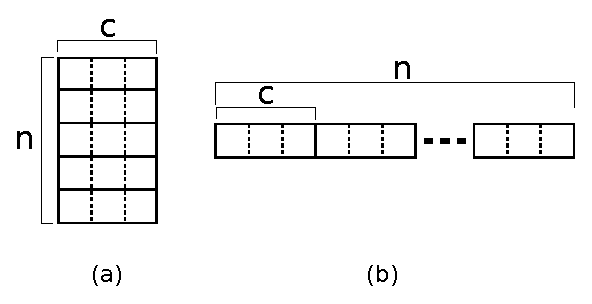
\includegraphics{figures/vectors}
%   \caption{View of  a Vector of size  n and c compenents,  (a) representation of
%     the vector, (b) representation of the storage of the same Vector.}
%   \label{fig:vectors}
% \end{figure}

% All the  data are linerarized  in memory in  an array called values.  This class
% member is public.  So for a Vector  of size $n$ and $c$ component, to access the
% $j^{th}$  component of  th  $i^{th}$ tuple,  you have  to  get $values[i  * c  +
% j]$. You  can also  access to this  value with  accessor \code{at(i, j)}  or the
% constant accessor \code{get(i, j)}.

% If  you want to  store a  matrix on  each tuple  you have  to linearize  it. For
% exemple if you want to store a m * k matrix on each tuple you must specify c = m
% * k.  To access a particular value  in a matrix of  a tuple you will  have to do
% something like $values[ i * m * k + j_i * m + j_j]$.

% \subsubsection{Vector storage convention within FE object\label{sec:FE-convention}}

% The point of  this section is to describe the convention  of storage for vectors
% intented  to be  passed to  {\bf  FE} object  methods.  Indeed  a convention  of
% necessary  since gradient  operators or  integrtaion loops  will use  vectors as
% input and ouput.   Such vectors will be ordered with  a specific convention that
% we intend to describe now.

% For  vector objects,  the  size of  the vector  is  always the  number of  nodes
% associated.  The number  of components  is related  to the  order of  the tensor
% considered. For a scalar  field it is 1, for a vectorial  field, the size of the
% vector is the number of components. For a $m\times n$ matrix field the number of
% components is $m\times n$.

% One common operation  is the manipulation of continuum  fields at the quadrature
% point  positions.   Here  the  size   of  the  vector  is   $mn\_element  \times
% nb\_quad\_points$  and  the  number  of  components is  related  to  the  stored
% object.  For instance the  method \verb$interpolateOnQuadraturePoints()$  take a
% nodal field  stored in a  vector($n\_nodes$,$dim$) and return  a vector($n\_elem
% \times n\_quads$,$dim$).

% Basic gradient operations, like method \verb$gradientOnQuadraturePoints()$, will
% take  as input a  vector($n\_nodes$,$dim$) and  return a  vector($n\_elem \times
% n\_quads$,$dim \times spatial\_dimension$) where spatial dimension is the number
% of dimension in which the domain is embedded.

% In  the  same  way   the  integration  routines  expect  vector($n\_elem  \times
% n\_quads$,$dim$)  and  will  return vector($n\_elem$,$dim$).   For  non-Gaussian
% integrations, the input  by be direction a nodal field.   (At present time, only
% gaussian integrators are implemented within akantu).

% Last but  not the least  is the vectorial  assembly process for which  accept as
% input vector($n\_elem \times n\_quads \times n\_nodes\_per\_element$,$dim$)
% and will return a vector($n\_nodes$,$dim$) nodal object.\\

% {\bf The general convention is that  the number of component shall always be the
%   size of  the object manipulated  at the lowest  level.  The object could  be a
%   per-element, of  per quadrature point  or even per  node basis this  will also
%   apply    as   shown    below.   The    figures    \ref{fig:vector-chain}   and
%   \ref{fig:interpolate-storage} shows the  pattern of the vectors is  the case a
%   interpolation on quadrature points.}

% \begin{figure}
%   \begin{equation}
%     \left(
%       \begin{array}{c}
%         N_1 \\
%         \vdots \\
%         N_I
%         \left\{
%           \begin{array}{c}
%             a_1 \\
%             \vdots \\
%             a_{dim} \\
%           \end{array}
%         \right. \\
%         \vdots \\
%         N_{nb\_nodes}
%       \end{array}
%     \right)
%     \begin{array}{c}
%       \Longrightarrow \\
%       interpolate\\
%       On\\
%       Quadrature\\
%       Points\\
%     \end{array}
%     \left(
%       \begin{array}{c}
%         E_1 \\
%         \vdots \\
%         E_e
%         \left\{
%           \begin{array}{c}
%             q_1 \\
%             \vdots \\
%             \left.
%               \begin{array}{c}
%                 a_1 \\
%                 \vdots \\
%                 a_{dim}
%               \end{array}
%             \right\} q_i \\
%             \vdots \\
%             q_p \\
%           \end{array}
%         \right.  \\
%         \vdots \\
%         E_{nb\_elements}
%       \end{array}
%     \right)
%   \end{equation}
%   \caption{\label{fig:vector-chain}Pattern   of   vectors   manipulated   during
%     interpolation on  quadrature points.  Symbols  N (resp. E, q)  denotes nodes
%     (resp. elements, quadrature points).}
% \end{figure}

% \begin{figure}[!htb]
%   \centering
%   \includegraphics[width=\textwidth]{figures/interpolate}
%   \caption{Input and output  vector of interpolateOnQuadraturePoints. The output
%     Vector has nb\_quadrature\_points tuples,  the quadrature points are grouped
%     by elements (p is the number of quadrature points per element).}
%   \label{fig:interpolate-storage}
% \end{figure}


% The planning to write the documentation
%\input{manual-planning}

% The documentation chapter (split in parts)
\chapter{Getting started}
\section{Downloading the code}

The \akantu source code can be requested using the form accessible at the URL
\url{http://lsms.epfl.ch/akantu}.  There, you will be asked to accept the LGPL
license terms.

\section{Compiling Akantu}

Akantu is a \code{cmake} project, so to configure it you can either follow the usual way:
\begin{command}
  > cd akantu
  > mkdir build
  > cd build
  > ccmake ..
  [ Set the options that you need ]
  > make
  > make install
\end{command}

Or, you can use a tool  we added to help you. You can just use the
given \code{Makefile} that handles the \code{cmake} configuration

\begin{command}
  > cd akantu
  > make config
  > make
  > make install
\end{command}

\section{Writing a \code{main} function\label{sect:common:main}}

First of all, \akantu needs to be initialized.  There is a memory
management included in the core library which allows a correct
allocation and de-allocation of vectors, structures and
objects. Moreover, in parallel computations the initialization
procedure can perform the communication setup. This is achieved by
 a pair of functions (\code{initialize} and \code{finalize})
that are used as follows:
\begin{cpp}
int main(int argc, char *argv[])
{
  akantu::initialize(argc, argv);

  // your code
  ...

  akantu::finalize();
}
\end{cpp}
The \code{initialize} function takes the program parameters which
can be interpreted by \akantu and given to the underlying libraries (\eg MPI).

\section{Creating and loading a mesh\label{sect:common:mesh}}

\akantu supports meshes generated with Gmsh~\cite{gmsh2009}, a free
software available at \url{http://geuz.org/gmsh/}. A detailed
documentation can be found at this URL, so this manual will not provide
Gmsh usage directions. Gmsh outputs meshes in \code{.msh} format that can be read
by \akantu. In order to import a mesh, it is necessary to create
a \code{Mesh} object through the following function calls:
\begin{cpp}
  UInt spatial_dimension = 2;
  Mesh mesh(spatial_dimension);
\end{cpp}
The only parameter that has to be specified by the user is the spatial
dimension of the problem. Now it is possible to read a \code{.msh} file with
a \code{read()} function of the mesh.
\begin{cpp}
  mesh.read("square.msh", mesh);
\end{cpp}
This function tries to guess the reader to use based on the extension of the file.

The mesh can also be wrote to a file with the \code{write()} method.
\begin{cpp}
  mesh.write("square_modified.msh", mesh);
\end{cpp}

For now, \akantu supports only meshes generated Gmsh or by
DIANA (\url{http://tnodiana.com}). If the \code{read()} or \code{write()}
functions cannot guess the file type, an optional parameter can be specified
to force the use of a particular reader/writer.

\begin{center}
  \begin{tabular}{lll}
    \toprule
    Mesh Type & \multicolumn{1}{c}{Key} & Capabilities\\
    \midrule
    Gmsh & \code{\_miot\_gmsh} & read/write\\
    Diana & \code{\_miot\_diana} & read\\
    \bottomrule
  \end{tabular}
\end{center}


\section{Using \code{Vectors}}

Data in \akantu can be stored in the data structures implemented by
the \code{Vector} class. In its most basic usage the \code{Vector} class
implemented in \akantu is similar to the \code{vector} class of
the Standard Template Library (STL) for C++. A simple \code{Vector}
containing a sequence of \code{nb\_element} values can be generated with:
\begin{cpp}
  Vector<type> example_vector(nb_element);
\end{cpp}
where \code{type} usually is \code{Real}, \code{UInt} or
\code{bool}. Each value is associated to an index, so that data can be
accessed by typing:

\begin{cpp}
  type & val = example_vector(index)
\end{cpp}

\code{Vectors} can also contain a sequence of values for each
index. In that case the number of components of each sequence must be
specified during \code{Vector} creation.  For example, if we want to
create a \code{Vector} to store the coordinates (sequence of three
values) of ten nodes, the appropriate code is the following:
\begin{cpp}
  UInt nb_nodes = 10;
  UInt spatial_dimension = 3;

  Vector<Real> position(nb_nodes, spatial_dimension);
\end{cpp}
In this case the $x$ position of node number 8 will be given by
\code{position(7, 0)} (in C++, numbering starts from 0). If the number of
components for the sequence is not specified, the default value of 1 is used.

It is very common in \akantu to loop over vectors to perform a specific
operation. This ranges from geometric calculation on nodal quantities
to tensor algebra (in constitutive laws for example).

The \code{Vector} object provides iterators
in order to make the writing of loops easier and enhance readability.
For instance, a loop over the nodal coordinates can be performed as:
\begin{cpp}
  //accessing the nodal coordinates Vector
  Vector<Real> & nodes = mesh.getNodes();

  //creating the iterators
  Vector<Real>::iterator<types::RVector> it  = nodes.begin(spatial_dimension);
  Vector<Real>::iterator<types::RVector> end = nodes.end(spatial_dimension);

  for (; it != end; ++it){
    RVector & coords = (*it);

    //do what you need
    ....
  }
\end{cpp}
In this example, each \code{RVector} is a geometrical vector of size \code{spatial\_dimension}
and the iteration is conveniently performed by the \code{Vector} iterator \code{it}.

The \code{Vector} object is intensively used to store tensor values.  In that
case it should be specified that the returned object type is a matrix when
constructing the iterator. This is done when calling the \code{begin} function. For
instance, assuming that we have a \code{Vector} storing stresses, we can loop
over the stored tensors by:

\begin{cpp}
  //creating the iterators
  Vector<Real>::iterator<types::RMatrix> it  = stresses.begin(spatial_dimension,spatial_dimension);
  Vector<Real>::iterator<types::RMatrix> end = stresses.end(spatial_dimension,spatial_dimension);

  for (; it != end; ++it){
    Matrix<Real> & stress = (*it);

    //do what you need
    ....
  }
\end{cpp}
In this last example, the \code{Matrix} objects have dimension
\code{spatial\_dimension} $\times$ \code{spatial\_dimension}.
The light objects \code{Matrix} and \code{RVector} can be used and combined
to do most common linear algebra.

In general, a mesh consists of several kinds of elements. Consequently, the
amount of data to be stored can differ for each element type. The straightforward
example is the connectivity array, \ie the sequences of nodes belonging to
each element. In order to easily manage this kind of data, a
particular data structure called \code{ByElementTypeVector} is available.
This structure is just a group of \code{Vector}, each associated to an element
type. The following code can retrieve the \code{ByElementTypeVector}
which stores the connectivity arrays for a mesh:
\begin{cpp}
  ByElementTypeVector<UInt> & connectivities = mesh.getConnectivities();
\end{cpp}
Then the specific vector associated to a given element type can be
obtained by
\begin{cpp}
  Vector<UInt> & connectivity_triangle = connectivities(_triangle_3);
\end{cpp}
where the first order 3-node triangular element was used in the presented
piece of code.

%%% Local Variables:
%%% mode: latex
%%% TeX-master: "manual"
%%% End:

\section{Elements\index{Elements}}

The base for every finite element computation is its mesh and the elements that are used within that mesh. What kind of element types can be used depends on the mesh, but also on the dimensionality of the problem (1D, 2D or 3D). In \akantu several isoparametric Langrangian element types are supported. Each of these types is discussed in more detail below, starting with the 1D-elements all the way to the 3D-elements. For each element type the coordinates of the nodes are given in the isoparametric frame of reference, together with the shape functions (and their derivatives) on these respective nodes. Also all the quadrature points within each element are listed (together with the weight that is applied on these points).

%%%%%%%%%% 1D %%%%%%%%%
\subsection{Isoparametric Elements in 1D\index{Elements!1D}}

In \akantu there are two types of isoparametric elements defined in 1D. These element types are called \code{segment\_2} and \code{segment\_3}.

\subsubsection{Segment 2\index{Elements!1D!Segment 2}}

\begin{Element}{1D}
 1  &  -1  &  $\half\left(1-\xi\right)$  &  $-\half$  & &\\
\elemline
 2  &   1  &  $\half\left(1+\xi\right)$  &  $\half$   & &\\
\end{Element}

\begin{QuadPoints}{1}
Coord. \elemcooroned  &  0  \\
\elemline
Weight  &  2  \\
\end{QuadPoints}

\subsubsection{Segment 3\index{Elements!1D!Segment 3}}

\begin{Element}{1D}
 1  &  -1  &  $\half\xi\left(\xi-1\right)$  &  $\xi-\half$   & &\\
\elemline
 2  &   1  &  $\half\xi\left(\xi+1\right)$  &  $\xi+\half$   & &\\
\elemline
 3  &   0  &  $1-\xi^{2}$                    &  $-2\xi$       & &\\
\end{Element}

\begin{QuadPoints}{2}
Coord. \elemcooroned  &  $-1/\sqrt{3}$  &  $1/\sqrt{3}$  \\
\elemline
Weight  &  1  &  1  \\
\end{QuadPoints}

%%%%%%%%%% 2D %%%%%%%%%
\subsection{Isoparametric Elements in 2D\index{Elements!2D}}

In \akantu there are four types of isoparametric elements defined in 2D. These element types are called \code{triangle\_3}, \code{triangle\_6}, \code{quadrangle\_4} and \code{quadrangle\_8}.

\subsubsection{Triangle 3\index{Elements!2D!Triangle 3}}

\begin{Element}{2D}
 1  &  0,0  &  $1-\xi-\eta$  &  -1  &  -1  & \\
\elemline
 2  &  1,0  &  $\xi$         &   1  &   0  & \\
\elemline
 3  &  0,1  &  $\eta$        &   0  &   1  & \\
\end{Element}

\begin{QuadPoints}{1}
Coord. \elemcoortwod  &  (\third,\third)  \\
\elemline
Weight  &  1  \\
\end{QuadPoints}

\subsubsection{Triangle 6\index{Elements!2D!Triangle 6}}

\begin{Element}{2D}
 1  &  0     , 0      &  $-\left(1-\xi-\eta\right)\left(1-2\left(1-\xi-\eta\right)\right)$ & $1-4\left(1-\xi-\eta\right)$ & $1-4\left(1-\xi-\eta\right)$ & \\
\elemline
 2  &  1     , 0      &  $-\xi\left(1-2\xi\right)$                                         & $4\xi-1$                     & $0$                          & \\
\elemline
 3  &  0     , 1      &  $-\eta\left(1-2\eta\right)$                                       & $0$                          & $4\eta-1$                    & \\
\elemline
 4  &  \half , 0      &  $4\xi\left(1-\xi-\eta\right)$                                     & $4\left(1-2\xi-\eta\right)$  & $-4\xi$                      & \\
\elemline
 5  &  \half , \half  &  $4\xi\eta$                                                        & $4\eta$                      & $4\xi$                       & \\
\elemline
 6  &  0     , \half  &  $4\eta\left(1-\xi-\eta\right)$                                    & $-4\eta$                     & $4\left(1-\xi-2\eta\right)$  & \\
\elemline
\end{Element}

\begin{QuadPoints}{3}
Coord. \elemcoortwod  &  (\sixth,\sixth) & (\twothird,\sixth) & (\sixth,\twothird) \\
\elemline
Weight & \sixth & \sixth & \sixth \\
\end{QuadPoints}

\subsubsection{Quadrangle 4\index{Elements!2D!Quadrangle 4}}

\begin{Element}{2D}
 1  &  -1 , -1  &  $\quart\left(1-\xi\right)\left(1-\eta\right)$  &  $-\quart\left(1-\eta\right)$  &  $-\quart\left(1-\xi\right)$ & \\
\elemline
 2  &   1 , -1  &  $\quart\left(1+\xi\right)\left(1-\eta\right)$  &  $\quart\left(1-\eta\right)$   &  $-\quart\left(1-\xi\right)$ & \\
\elemline
 3  &   1 ,  1  &  $\quart\left(1+\xi\right)\left(1+\eta\right)$  &  $\quart\left(1-\eta\right)$   &  $\quart\left(1-\xi\right)$  & \\
\elemline
 4  &  -1 ,  1  &  $\quart\left(1-\xi\right)\left(1+\eta\right)$  &  $-\quart\left(1-\eta\right)$  &  $\quart\left(1-\xi\right)$  & \\
\end{Element}

\begin{QuadPoints}{4}
Coord. \elemcoortwod  &  ($-1/\sqrt{3}$,$-1/\sqrt{3}$)  &  ($1/\sqrt{3}$,$-1/\sqrt{3}$)  &  ($1/\sqrt{3}$,$1/\sqrt{3}$)  & ($-1/\sqrt{3}$,$1/\sqrt{3}$) \\ 
\elemline
Weight & 1 & 1 & 1 & 1 \\
\end{QuadPoints}

\subsubsection{Quadrangle 8\index{Elements!2D!Quadrangle 8}}

\begin{Element}{2D}
 1  &  -1 , -1  &  $\quart\left(1-\xi\right)\left(1-\eta\right)\left(-1-\xi-\eta\right)$ 
                &  $\quart\left(1-\eta\right)\left(2\xi+\eta\right)$
                &  $\quart\left(1-\xi\right)\left(\xi+2\eta\right)$  & \\
\elemline
 2  &   1 , -1  &  $\quart\left(1+\xi\right)\left(1-\eta\right)\left(-1+\xi-\eta\right)$ 
                &  $\quart\left(1-\eta\right)\left(2\xi-\eta\right)$
                &  $-\quart\left(1+\xi\right)\left(\xi-2\eta\right)$  & \\
\elemline
 3  &   1 ,  1  &  $\quart\left(1+\xi\right)\left(1+\eta\right)\left(-1+\xi+\eta\right)$ 
                &  $\quart\left(1+\eta\right)\left(2\xi+\eta\right)$
                &  $\quart\left(1+\xi\right)\left(\xi+2\eta\right)$  & \\
\elemline
 4  &  -1 ,  1  &  $\quart\left(1-\xi\right)\left(1+\eta\right)\left(-1-\xi+\eta\right)$ 
                &  $\quart\left(1+\eta\right)\left(2\xi-\eta\right)$
                &  $-\quart\left(1-\xi\right)\left(\xi-2\eta\right)$  & \\
\elemline
 5  &   0 , -1  &  $\half\left(1-\xi^{2}\right)\left(1-\eta\right)$ 
                &  $-\xi\left(1-\eta\right)$
                &  $-\half\left(1-\xi^{2}\right)$  & \\
\elemline
 6  &   1 ,  0  &  $\half\left(1+\xi\right)\left(1-\eta^{2}\right)$
                &  $\half\left(1-\eta^{2}\right)$
                &  $-\eta\left(1+\xi\right)$  & \\
\elemline
 7  &   0 ,  1  &  $\half\left(1-\xi^{2}\right)\left(1+\eta\right)$
                &  $-\xi\left(1+\eta\right)$
                &  $\half\left(1-\xi^{2}\right)$  & \\
\elemline
 8  &  -1 ,  0  &  $\half\left(1-\xi\right)\left(1-\eta^{2}\right)$
                &  $-\half\left(1-\eta^{2}\right)$
                &  $-\eta\left(1-\xi\right)$  & \\
\end{Element}

\begin{QuadPoints}{5}
Coord. \elemcoortwod & (0,0) & ($\sqrt{3/5}$,$\sqrt{3/5}$) & ($-\sqrt{3/5}$,$\sqrt{3/5}$) & ($-\sqrt{3/5}$,$-\sqrt{3/5}$) & ($\sqrt{3/5}$,$-\sqrt{3/5}$) \\
\elemline
Weight & 64/81 & 25/81 & 25/81 & 25/81 & 25/81 \\
\elemline
Coord. \elemcoortwod &         (0,$\sqrt{3/5}$)            & ($-\sqrt{3/5}$,0)            & (0,$-\sqrt{3/5}$)             & ($\sqrt{3/5}$,0) \\
\elemline
Weight & 40/81 & 40/81 & 40/81 & 40/81 \\
\end{QuadPoints}

%%%%%%%%%% 3D %%%%%%%%%
\subsection{Isoparametric Elements in 3D\index{Elements!3D}}

\subsubsection{Tetrahedron 4\index{Elements!3D!Tetrahedron 4}}

\subsubsection{Tetrahedron 10\index{Elements!3D!Tetrahedron 10}}

\subsubsection{Hexahedron 8\index{Elements!3D!Hexahedron 8}}


%\IfFileExists{manual-lumping.tex}{}{\input{manual-lumping}}

\chapter{Solid Mechanics Model\index{SolidMechanicsModel}\label{sect:smm}}

The solid mechanics model is a specific implementation of the
\code{Model} interface dedicated to handle the equations of motion or
equations of equilibrium. The model is created for a given mesh.  It
will create its own \code{FEEngine} object to compute the interpolation,
gradient, integration and assembly operations.  A
\code{SolidMechanicsModel} object can simply be created like this:
\begin{cpp}
  SolidMechanicsModel model(mesh, spatial_dimension);
\end{cpp}
where \code{mesh} is the mesh for which the equations are to be
solved, and \code{spatial\_dimension} is the dimensionality of the
problem.  If the \code{spatial\_dimension} is omitted, the problem is
assumed to have the same dimensionality as the one specified in the
mesh.

This model contains at least the the following six \code{Arrays}:
\begin{description}
\item[blocked\_dofs] contains a Boolean value for each degree of
  freedom specifying whether that degree is blocked or not. A
  Dirichlet boundary condition can be prescribed by setting the
  \textbf{blocked\_dofs} value of a degree of freedom to \code{true}.
  A Neumann boundary condition can be applied by setting the
  \textbf{blocked\_dofs} value of a degree of freedom to \code{false}.
  The \textbf{displacement}, \textbf{velocity} and
  \textbf{acceleration} are computed for all degrees of freedom for
  which the \textbf{blocked\_dofs} value is set to \code{false}. For
  the remaining degrees of freedom, the imposed values (zero by
  default after initialization) are kept.
\item[displacement] contains the displacements of all degrees of
  freedom. It can be either a computed displacement for free degrees
  of freedom or an imposed displacement in case of blocked ones
  ($\vec{u}$ in the following).
\item[velocity] contains the velocities of all degrees of freedom.  As
  \textbf{displacement}, it contains computed or imposed velocities
  depending on the nature of the degrees of freedom ($\vec{\dot{u}}$
  in the following).
\item[acceleration] contains the accelerations of all degrees of
  freedom. As \textbf{displacement}, it contains computed or imposed
  accelerations depending on the nature of the degrees of freedom
  ($\vec{\ddot{u}}$ in the following).
\item[force] contains the external forces applied on the nodes
  ($\vec{f_{\st{ext}}}$ in the following).
\item[residual] contains the difference between external and internal
  forces. On blocked degrees of freedom, \textbf{residual} contains
  the support reactions.  ($\vec{r}$ in the following).  It should be
  mentioned that at equilibrium \textbf{residual} should be zero on
  free degrees of freedom.
\end{description}

Some examples to help to understand how to use this model will be
presented in the next sections.

\section{Model Setup}


\subsection{Setting Initial Conditions \label{sect:smm:initial_condition}}

For a unique solution of the equations of motion, initial
displacements and velocities for all degrees of freedom must be
specified:
\begin{eqnarray}
  \vec{u(t=0)} = \vec{u}_{0}\\
  \vec{\dot u(t=0)} =\vec{v}_{0}
\end{eqnarray} The solid mechanics model can be initialized as
follows:
\begin{cpp}
  model.initFull()
\end{cpp}
This function initializes the internal arrays and sets them to
zero. Initial displacements and velocities that are not equal to zero
can be prescribed by running a loop over the total number of
nodes. Here, the initial displacement in $x$-direction and the
initial velocity in $y$-direction for all nodes is set to $0.1$ and $1$,
respectively.
\begin{cpp}
Array<Real> & disp = model.getDisplacement();
Array<Real> & velo = model.getVelocity();
for (UInt i = 0; i < nb_nodes; ++i) {
  disp(i, 0) = 0.1;
  velo(i, 1) = 1.;
}
\end{cpp}

\subsection{Setting Boundary Conditions\label{sect:smm:boundary}}
This section explains how to impose Dirichlet or Neumann boundary
conditions. A Dirichlet boundary condition specifies the values that
the displacement needs to take for every point $x$ at the boundary
($\Gamma_u$) of the problem domain (Fig.~\ref{fig:smm:boundaries}):
\begin{equation}
  \vec{u} = \vec{\bar u} \quad \forall \vec{x}\in
  \Gamma_{u}
\end{equation}
A Neumann boundary condition imposes the value of the gradient of the
solution at the boundary ($\Gamma_t$) of the problem domain
(Fig.~\ref{fig:smm:boundaries}):
\begin{equation}
  \vec{t} = \mat{\sigma} \vec{n} = \vec{\bar t} \quad
  \forall \vec{x}\in \Gamma_{t}
\end{equation}

\begin{figure} \centering
\def\svgwidth{0.5\columnwidth}
  \input{figures/problemDomain.pdf_tex}
  \caption{Problem domain $\Omega$ with boundary in three dimensions. The Dirchelet and the Neumann regions of the boundary are denoted with $\Gamma_u$ and $\Gamma_t$, respecitvely.\label{fig:smm:boundaries}}
  \label{fig:problemDomain}
\end{figure}

Different ways of imposing these boundary conditions exist. A basic
way is to loop over nodes or elements at the boundary and apply local
values. A more advanced method consists of using the notion of the
boundary of the mesh. In the following both ways are presented.

Starting with the basic approach, as mentioned, the Dirichlet boundary
conditions can be applied by looping over the nodes and assigning the
required values. Figure~\ref{fig:smm:dirichlet_bc} shows a beam with a
fixed support on the left side. On the right end of the beam, a load
is applied. At the fixed support, the displacement has a given
value. For this example, the displacements in both the $x$ and the
$y$-direction are set to zero. Implementing this displacement boundary
condition is similar to the implementation of initial displacement
conditions described above. However, in order to impose a displacement
boundary condition for all time steps, the corresponding nodes need to
be marked as boundary nodes as shown in the following code:

\begin{cpp}
Array<bool> & blocked = model.getBlockedDOFs();

const Array<Real> & pos = mesh.getNodes();

UInt nb_nodes = mesh.getNbNodes();
Real epsilon = Math::getTolerance();
/* this tolerance is by default equal to the machine precision but can be changed by using %\code{Math::setTolerance(value)}% */

for (UInt i = 0; i < nb_nodes; ++i) {
  if(std::abs(pos(i, 0)) < epsilon) {
    blocked(i, 0) = true; //block displacement in x-direction
    blocked(i, 1) = true; //block displacement in y-direction
    disp(i, 0) = 0.; //fixed displacement in x-direction
    disp(i, 1)= 0.; //fixed displacement in y-direction
  }
}
\end{cpp}

\begin{figure}[!htb]
  \centering
  \includegraphics[scale=0.4]{figures/dirichlet}
  \caption{Beam with fixed support.\label{fig:smm:dirichlet_bc}}
\end{figure}

For the more advanced approach, one needs the notion of a boundary in
the mesh. Therefore, the boundary should be created before boundary
condition functors can be applied. Generally the boundary can be
specified from the mesh file or the geometry.  For the first case, the
function \code{createGroupsFromMeshData} is called.  This function
can read any types of mesh data which are provided in the mesh
file. If the mesh file is created with Gmsh, the function takes one
input strings which is either \code{tag\_0}, \code{tag\_1} or
\code{physical\_names}. The first two tags are assigned by Gmsh to
each element which shows the physical group that they belong to. In
Gmsh, it is also possible to consider strings for different groups of
elements. These elements can be separated by giving a string
\code{physical\_names} to the function
\code{createGroupsFromMeshData}.  Boundary conditions can also be
created from the geometry by calling
\code{createBoundaryGroupFromGeometry}. This function gathers all the
elements on the boundary of the geometry.

To apply the required boundary conditions, the function \code{applyBC}
from the \code{SolidMechanicsModel} needs to be called. This function
gets a Dirichlet or Neumann functor and a string which specifies the
desired boundary on which the boundary conditions is to be
applied. The functors specify the type of conditions to apply. Three
built-in functors for Dirichlet exist: \code{FlagOnly, FixedValue,}
and \code{IncrementValue}. The functor \code{FlagOnly} is used if a
point is fixed in a given direction. Therefore, the input parameter to
this functor is only the fixed direction. The \code{FixedValue}
functor is used when a displacement value is applied in a fixed
direction. The \code{IncrementValue} applies an increment to the
displacement in a given direction. The following code shows the
utilization of three functors for the top, bottom and side surface of
the mesh which were already defined in the Gmsh file:

\begin{cpp}
mesh.createGroupsFromMeshData<std::string>("physical_names");

model.applyBC(BC::Dirichlet::FixedValue(13.0, BC::_y), "Top");

model.applyBC(BC::Dirichlet::FlagOnly(BC::_x), "Bottom");

model.applyBC(BC::Dirichlet::IncrementValue(13.0, BC::_x), "Side");
\end{cpp}

To apply a Neumann boundary condition, the applied traction or stress
should be specified before. In case of specifying the traction on the
surface, the functor \code{FromTraction} of Neumann boundary
conditions is called. Otherwise, the functor \code{FromStress} should
be called which gets the stress tensor as an input parameter.

\begin{cpp}
Array<Real> surface_traction(3);
surface_traction(0)=0.0;
surface_traction(1)=0.0;
surface_traction(2)=-1.0;

Array<Real> surface_stress(3, 3, 0.0);
surface_stress(0,0)=0.0;
surface_stress(1,1)=0.0;
surface_stress(2,2)=-1.0;

model.applyBC(BC::Neumann::FromTraction(surface_traction), "Bottom");

model.applyBC(BC::Neumann::FromStress(surface_stress), "Top");
\end{cpp}

If the boundary conditions need to be removed during the simulation, a
functor is called from the Neumann boundary condition to free those
boundary conditions from the desired boundary.

\begin{cpp}
 model.applyBC(BC::Neumann::FreeBoundary(), "Side");
\end{cpp}

User specified functors can also be implemented.  A full example for
setting both initial and boundary conditions can be found in
\shellcode{\examplesdir/boundary\_conditions.cc}.  The problem solved
in this example is shown in Fig.~\ref{fig:smm:bc_and_ic}. It consists
of a plate that is fixed with movable supports on the left and bottom
side. On the right side, a traction, which increases linearly with the
number of time steps, is applied. The initial displacement and
velocity in $x$-direction at all free nodes is zero and two
respectively.
\begin{figure}[!htb]
  \centering
  \includegraphics[scale=0.8]{figures/bc_and_ic_example}
  \caption{Plate on movable supports.\label{fig:smm:bc_and_ic}}
\end{figure}

\subsection{Material Selector\label{sect:smm:materialselector}}

If the user wants to assign different materials to the different
finite elements of choice in \akantu, a material selector has to be
used. There are four different material selectors pre-defined in
\akantu.

\begin{enumerate}
\item \code{MaterialSelector}: This material selector assigns a
  material to a specific element using an index value. If an index is
  not specified, it is using \code{0}, hence the first material as
  default.
\item \code{DefaultMaterialSelector}: This selector assigns materials
  based on the values in the \code{element\_index\_by\_material}
  array.
\item \code{MeshDataMaterialSelector}: This material selector class
  uses mesh data information to assign different materials. With the
  proper tag name and index, different materials can be assigned as
  demonstrated in the example below.
\item \code{DefaultMaterialCohesiveSelector}: This is the default
  material selector for the cohesive elements and it inherits its
  properties from \code{DefaultMaterialSelector}. The material ID of
  the first cohesive element is extracted and assigned to all cohesive
  elements.
\end{enumerate}

Apart from the \akantu's default material selectors, users can always
develop their own classes in the main code to tackle various
multi-material assignment situations.

For example, an application of \code{MeshDataMaterialSelector} could
look like this:

\begin{cpp}
  MeshDataMaterialSelector<std::string> * mat_selector;
  mat_selector = new MeshDataMaterialSelector<std::string>("physical_names", model);
  model.setMaterialSelector(*mat_selector);
\end{cpp}

In this example the physical names specified in a GMSH geometry file will by
used to match the material names in the input file.

Another example would be:

\begin{cpp}
  MeshDataMaterialSelector<UInt> * mat_selector;
  mat_selector = new MeshDataMaterialSelector<UInt>("tag_1", model);
  model.setMaterialSelector(*mat_selector);
\end{cpp}

where \code{tag\_1} of the mesh file is used as the classifier index
and the elements that have index value equal to one will be assigned
to the second material in the material file.

\IfFileExists{manual-cohesive_elements_insertion.tex}{\subsection{Insertion of cohesive elements}
When the intrinsic approach is chosen, cohesive elements are to be
inserted just after reading the mesh by using the
\code{CohesiveElementInserter} class. Here an example is given:
\begin{cpp}
  CohesiveElementInserter inserter(mesh);
  inserter.setLimit('x', -1, 1);
  inserter.insertIntrinsicElements();
\end{cpp}
First the element inserter is created and then the insertion is
limited to the range $[-1,1]$ in $x$ direction. Additional ranges in
$y$ and $z$ directions can be added as well. In this way cohesive
elements are inserted only on those facets whose barycenter is inside
the ranges. Then the \code{insertIntrinsicElements} can be called.

Then a cohesive model should be created and initialized as
\begin{cpp}
  SolidMechanicsModelCohesive model(mesh);
  model.initFull("material.dat");
\end{cpp}

When extrinsic simulations are carried out, the model should be
initialized as follows:
\begin{cpp}
  SolidMechanicsModelCohesive model(mesh);
  model.initFull("material.dat", SolidMechanicsModelCohesiveOptions(_explicit_lumped_mass, true));
\end{cpp}
In order to check stress for automatic element insertion it is
necessary to call the following function in the main loop:
\begin{cpp}
  model.checkCohesiveStress();
\end{cpp}
By default the check is performed on all facet, but it can be
restricted by providing ranges as for intrinsic element insertion. The
cohesive model for extrinsic simulations has an element inserter that
can be called:
\begin{cpp}
  CohesiveElementInserter & inserter = model.getElementInserter();
  inserter.setLimit('y', 0.5, 3);
  model.updateAutomaticInsertion();
\end{cpp}

Anytime during the simulation it is possible to access the following
energies with the relative function:
\begin{cpp}
  Real Ed = model.getEnergy("dissipated");
  Real Er = model.getEnergy("reversible");
  Real Ec = model.getEnergy("contact");
\end{cpp}
}{}

\section{Static Analysis\label{sect:smm:static}}

The \code{SolidMechanicsModel} class can handle different analysis
methods, the first one being presented is the static case.  In this
case, the equation to solve is,
\begin{equation}
  \label{eqn:smm:static} \mat{K} \vec{u} =
  \vec{f_{\st{ext}}}~,
\end{equation}
where $\mat{K}$ is the global stiffness matrix, $\vec{u}$ the
displacement vector and $\vec{f_{\st{ext}}}$ the vector of external
forces applied to the system.

To solve such a problem, the static solver of the
\code{SolidMechanicsModel}\index{SolidMechanicsModel} object is used.
First, a model has to be created and initialized.  To create the
model, a mesh (which can be read from a file) is needed, as explained
in Section~\ref{sect:common:mesh}.  Once an instance of a
\code{SolidMechanicsModel} is obtained, the easiest way to initialize
it is to use the \code{initFull}\index{SolidMechanicsModel!initFull}
method by giving the \code{SolidMechanicsModelOptions}. These options
specify the type of analysis to be performed and whether the materials
should be initialized or not.
\begin{cpp}
SolidMechanicsModel model(mesh);
model.initFull(SolidMechanicsModelOptions(_static));
\end{cpp}
Here, a static analysis is chosen by passing the argument
\code{\_static} to the method. By default, the Boolean for no
initialization of the materials is set to false, so that they are
initialized during the \code{initFull}. The method \code{initFull}
also initializes all appropriate vectors to zero.  Once the model is
created and initialized, the boundary conditions can be set as
explained in Section~\ref{sect:smm:boundary}.  Boundary conditions
will prescribe the external forces for some free degrees of freedom
$\vec{f_{\st{ext}}}$ and displacements for some others.  At this point
of the analysis, the function
\code{solveStep}\index{SolidMechanicsModel!solveStep} can be called:
\begin{cpp}
model.solveStep<_scm_newton_raphson_tangent_modified, _scc_residual>(1e-4, 1);
\end{cpp}
This function is templated by the solving method and the convergence
criterion and takes two arguments: the tolerance and the maximum
number of iterations, which are $1e-4$ and $1$ for this example. The
modified Newton-Raphson method is chosen to solve the system. In this
method, the equilibrium equation (\ref{eqn:smm:static}) is modified in
order to apply a Newton-Raphson convergence algorithm:

\begin{align}\label{eqn:smm:static-newton-raphson}
\mat{K}^{i+1}\delta\vec{u}^{i+1} &= \vec{r} \\
&= \vec{f_{\st{ext}}} -\vec{f_{\st{int}}}\\
&= \vec{f_{\st{ext}}} - \mat{K}^{i} \vec{u}^{i}\\
\vec{u}^{i+1} &= \vec{u}^{i} + \delta\vec{u}^{i+1}~,\nonumber
\end{align}
where $\delta\vec{ u}$ is the increment of displacement to be added
from one iteration to the other, and $i$ is the Newton-Raphson
iteration counter.  By invoking the \code{solveStep} method in the
first step, the global stiffness matrix $\mat{K}$ from
Equation~(\ref{eqn:smm:static}) is automatically assembled. A
Newton-Raphson iteration is subsequently started, $\mat{K}$ is updated
according to the displacement computed at the previous iteration and
one loops until the forces are balanced (\code{\_scc\_residual}), \ie
$||\vec{r}|| < \mbox{\code{\_scc\_residual}}$.  One can also iterate
until the increment of displacement is zero (\code{\_scc\_increment})
which also means that the equilibrium is found.  For a linear elastic
problem, the solution is obtained in one iteration and therefore the
maximum number of iterations can be set to one. But for a non-linear
case, one needs to iterate as long as the norm of the residual exceeds
the tolerance threshold and therefore the maximum number of iterations
has to be higher, e.g.  $100$:
\begin{cpp}
model.solveStep<_scm_newton_raphson_tangent_modified,_scc_residual>(1e-4, 100);
\end{cpp}
At the end of the analysis, the final solution is stored in the
\textbf{displacement} vector.  A full example of how to solve a static
problem is presented in the code \code{\examplesdir/static/static.cc}.
This example is composed of a 2D plate of steel, blocked with rollers
on the left and bottom sides as shown in Figure \ref{fig:smm:static}.
The nodes from the right side of the sample are displaced by $0.01\%$
of the length of the plate.

\begin{figure}[!htb]
  \centering
  \includegraphics{figures/static}
  \caption{Numerical setup\label{fig:smm:static}}
\end{figure}

The results of this analysis is depicted in
Figure~\ref{fig:smm:implicit:static_solution}.

\begin{figure}[!htb]
  \centering
  \includegraphics[width=.6\linewidth]{figures/static_analysis}
  \caption{Solution of the static analysis. Left: the initial
condition, right: the solution (deformation magnified 50 times)}
  \label{fig:smm:implicit:static_solution}
\end{figure}

\section{Dynamic Methods} \label{sect:smm:Dynamic_methods}

Different ways to solve the equations of motion are implemented in the
solid mechanics model.  The complete equations that should be solved
are:
\begin{equation}
\label{eqn:equation-motion}
\mat{M}\vec{\ddot{u}} +
\mat{C}\vec{\dot{u}} + \mat{K}\vec{u} = \vec{f_{\st{ext}}}~,
\end{equation}
where $\mat{M}$, $\mat{C}$ and $\mat{K}$ are the mass,
damping and stiffness matrices, respectively.

In the previous section, it has already been discussed how to solve
this equation in the static case, where $\vec{\ddot{u}} =
\vec{\dot{u}} = 0$.  Here the method to solve this equation in the
general case will be presented.  For this purpose, a time
discretization has to be specified.  The most common discretization
method in solid mechanics is the Newmark-$\beta$ method, which is
also the default in \akantu.

For the Newmark-$\beta$ method, (\ref{eqn:equation-motion}) becomes a
system of three equations (see \cite{curnier92a} \cite{hughes-83a} for
more details):
\begin{align}
\mat{M} \vec{\ddot{u}}_{n+1} + \mat{C}\vec{\dot{u}}_{n+1} + \mat{K} \vec{u}_{n+1} &=\vec{f_{\st{ext}}}_{n+1}
\label{eqn:equation-motion-discret} \\
\vec{u}_{n+1} &=\vec{u}_{n} + \left(1 - \alpha\right) \Delta t \vec{\dot{u}}_{n} +
\alpha \Delta t \vec{\dot{u}}_{n+1} + \left(\frac{1}{2} -
\alpha\right) \Delta t^2
\vec{\ddot{u}}_{n} \label{eqn:finite-difference-1}\\
\vec{\dot{u}}_{n+1} &= \vec{\dot{u}}_{n} + \left(1 - \beta\right)
\Delta t \vec{\ddot{u}}_{n} + \beta \Delta t
\vec{\ddot{u}}_{n+1} \label{eqn:finite-difference-2}
\end{align}

In these new equations, $\vec{\ddot{u}}_{n}$, $\vec{\dot{u}}_{n}$ and
$\vec{u}_{n}$ are the approximations of $\vec{\ddot{u}(t_n)}$,
$\vec{\dot{u}(t_n)}$ and $\vec{u(t_n)}$.
Equation~(\ref{eqn:equation-motion-discret}) is the equation of motion
discretized in space (finite-element discretization), and equations
(\ref{eqn:finite-difference-1}) and (\ref{eqn:finite-difference-2})
are discretized in both space and time (Newmark discretization).  The
$\alpha$ and $\beta$ parameters determine the stability and the
accuracy of the algorithm. Classical values for $\alpha$ and $\beta$
are usually $\beta = 1/2$ for no numerical damping and $0 < \alpha <
1/2$.

\begin{center}
  \begin{tabular}{cll}
    \toprule
    $\alpha$ & Method ($\beta = 1/2$) & Type\\
    \midrule
    $0$ & central difference & explicit\\
    $1/6$ & Fox-Goodwin (royal road) &implicit\\
    $1/3$ & Linear acceleration &implicit\\
    $1/2$ & Average acceleration (trapezoidal rule)& implicit\\
    \bottomrule
  \end{tabular}
\end{center}

The solution of this system of equations,
(\ref{eqn:equation-motion-discret})-(\ref{eqn:finite-difference-2}) is
split into a predictor and a corrector system of equations.  Moreover,
in the case of a non-linear equations, an iterative algorithm such as
the Newton-Raphson method is applied. The system of equations can be
written as:


\noindent\textit{Predictor:}
\begin{align}
  \vec{u}_{n+1}^{0} &= \vec{u}_{n} + \Delta t
  \vec{\dot{u}}_{n} + \frac{\Delta t^2}{2} \vec{\ddot{u}}_{n} \\
  \vec{\dot{u}}_{n+1}^{0} &= \vec{\dot{u}}_{n} + \Delta t
  \vec{\ddot{u}}_{n} \\
  \vec{\ddot{u}}_{n+1}^{0} &= \vec{\ddot{u}}_{n}
\end{align}

\noindent\textit{Solve:}
\begin{align}
  \left(c \mat{M} + d \mat{C} + e \mat{K}_{n+1}^i\right)
  \vec{w} = \vec{f_{\st{ext}}}_{n+1} - \vec{f_{\st{int}}}_{n+1}^i -
  \mat{C} \vec{\dot{u}}_{n+1}^i - \mat{M} \vec{\ddot{u}}_{n+1}^i = \vec{r}_{n+1}^i
\end{align}

\noindent\textit{Corrector:}
\begin{align}
  \vec{\ddot{u}}_{n+1}^{i+1} &= \vec{\ddot{u}}_{n+1}^{i} +c \vec{w} \\
  \vec{\dot{u}}_{n+1}^{i+1} &= \vec{\dot{u}}_{n+1}^{i} + d\vec{w} \\
  \vec{u}_{n+1}^{i+1} &= \vec{u}_{n+1}^{i} + e \vec{w}
\end{align}

where $i$ is the Newton-Raphson iteration counter and $c$, $d$ and $e$
are parameters depending on the method used to solve the equations

\begin{center}
  \begin{tabular}{lcccc}
    \toprule
    & $\vec{w}$ & $e$ & $d$ & $c$\\
    \midrule
    in acceleration &$ \delta\vec{\ddot{u}}$ & $\alpha \beta\Delta t^2$ &$\beta \Delta t$ &$1$\\
    in velocity & $ \delta\vec{\dot{u}}$& $\frac{1}{\beta} \Delta t$ & $1$ & $\alpha\Delta t$\\
    in displacement &$\delta\vec{u}$ & $ 1$ & $\frac{1}{\alpha} \Delta t$ & $\frac{1}{\alpha \beta} \Delta t^2$\\
    \bottomrule
  \end{tabular}
\end{center}

%\note{If you want to use the implicit solver \akantu should be compiled at least with one sparse matrix solver such as Mumps\cite{mumps}.}


\subsection{Implicit Time Integration}
To solve a problem with an implicit time integration scheme, first a
\code{SolidMechanicsModel} object has to be created and initialized.
Then the initial and boundary conditions have to be set.  Everything
is similar to the example in the static case
(Section~\ref{sect:smm:static}), however, in this case the implicit
dynamic scheme is selected at the initialization of the model.

\begin{cpp}
SolidMechanicsModel model(mesh);
model.initFull(SolidMechanicsModelOptions(_implicit_dynamic));
/*Boundary conditions see Section~%\ref{sect:smm:boundary}% */
\end{cpp}
Because a dynamic simulation is conducted, an integration time step
$\Delta t$ has to be specified. In the case of implicit simulations,
\akantu implements a trapezoidal rule by default.  That is to say
$\alpha = 1/2$ and $\beta = 1/2$ which is unconditionally
stable. Therefore the value of the time step can be chosen arbitrarily
within reason.  \index{SolidMechanicsModel!setTimeStep}
\begin{cpp}
model.setTimeStep(time_step);
\end{cpp}
Since the system has to be solved for a given amount of time, the
method \code{solveStep()}, (which has already been used in the static
example in Section~\ref{sect:smm:static}), is called inside a time
loop:
\begin{cpp}
/// time loop
Real time = 0.;
for (UInt s = 1; time <max_time; ++s, time += time_step) {
  model.solveStep<_scm_newton_raphson_tangent_modified,_scc_increment>(1e-12, 100);
}
\end{cpp}
An example of solid mechanics with an implicit time integration scheme
is presented in
\shellcode{\examplesdir/implicit/implicit\_dynamic.cc}.  This example
consists of a 3D beam of
$\unit{10}{\meter}\,\times\,\unit{1}{\meter}\,\times\,\unit{1}{\meter}$
blocked on one side and is on a roller on the other side.  A constant
force of \unit{5}{\kilo\newton} is applied in its middle.
Figure~\ref{fig:smm:implicit:dynamic} presents the geometry of this
case. The material used is a fictitious linear elastic material with a
density of \unit{1000}{\kilogrampercubicmetre}, a Young's Modulus of
\unit{120}{\mega\pascal} and Poisson's ratio of $0.3$. These values
were chosen to simplify the analytical solution.

An approximation of the dynamic response of the middle point of the
beam is given by:
\begin{equation}
  \label{eqn:smm:implicit}
  u\left(\frac{L}{2}, t\right)
  = \frac{1}{\pi^4} \left(1 - cos\left(\pi^2 t\right) +
    \frac{1}{81}\left(1 - cos\left(3^2 \pi^2 t\right)\right) +
    \frac{1}{625}\left(1 - cos\left(5^2 \pi^2 t\right)\right)\right)
\end{equation}

\begin{figure}[!htb]
  \centering
  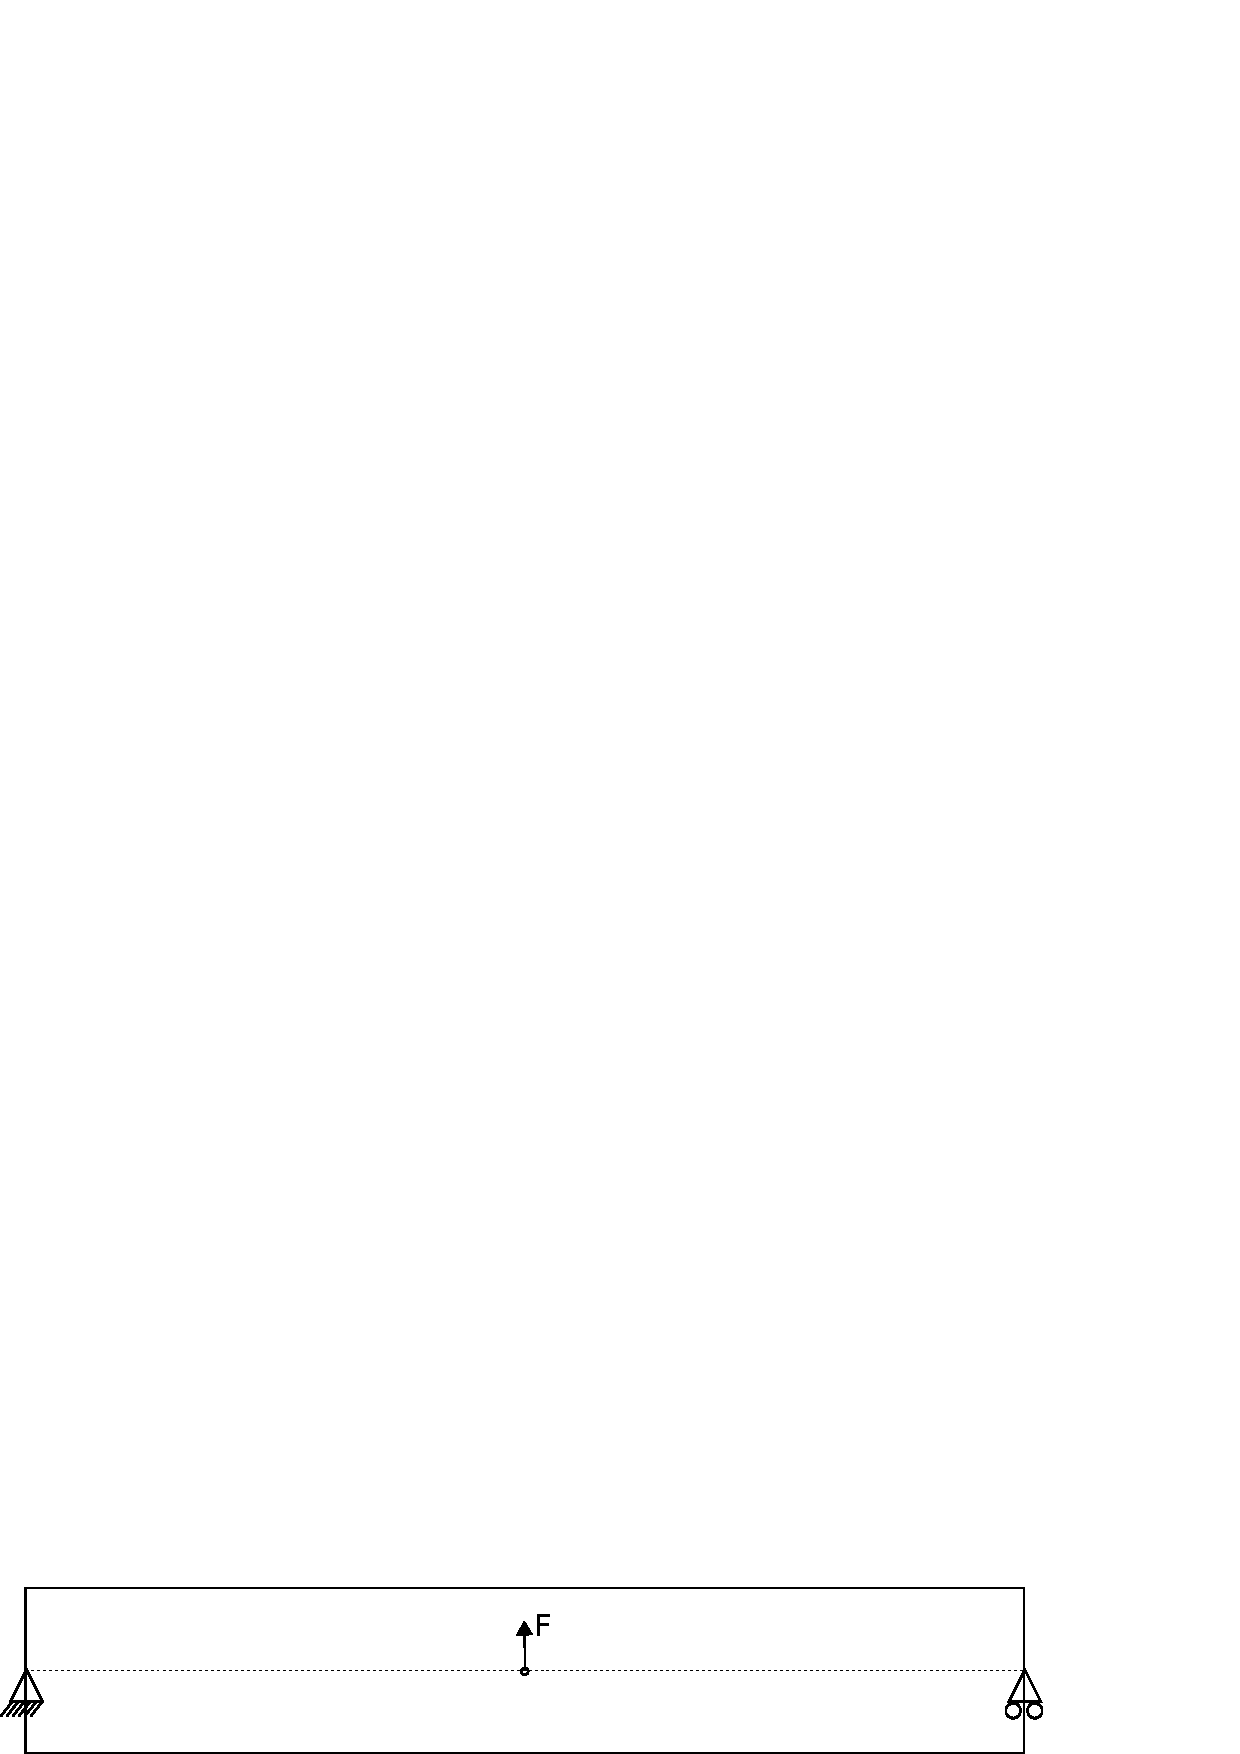
\includegraphics[scale=.6]{figures/implicit_dynamic}
  \caption{Numerical setup}
  \label{fig:smm:implicit:dynamic}
\end{figure}

Figure \ref{fig:smm:implicit:dynamic_solution} presents the deformed
beam at 3 different times during the simulation: time steps 0, 1000 and
2000.

\begin{figure}[!htb]
  \centering
  \setlength{\unitlength}{0.1\textwidth}
  \begin{tikzpicture}
    \node[above right] (img) at (0,0)
    {\includegraphics[width=.6\linewidth]{figures/dynamic_analysis}};
    \node[left] at (0pt,20pt) {$0$}; \node[left] at (0pt,60pt) {$1000$};
    \node[left] at (0pt,100pt) {$2000$};
  \end{tikzpicture}

  \caption{Deformed beam at 3 different times (displacement are
    magnified by a factor 10).}
  \label{fig:smm:implicit:dynamic_solution}
\end{figure}

\subsection{Explicit Time Integration}

The explicit dynamic time integration scheme is based on the
Newmark-$\beta$ scheme with $\alpha=0$ (see equations
\ref{eqn:equation-motion-discret}-\ref{eqn:finite-difference-2}).  In
\akantu, $\beta$ is defaults to $\beta=1/2$, see section
\ref{sect:smm:Dynamic_methods}.

The initialization of the simulation is similar to the static and
implicit dynamic version.  The model is created from the
\code{SolidMechanicsModel} class.  In the initialization, the explicit
scheme is selected using the \code{\_explicit\_lumped\_mass} constant.

\begin{cpp}
SolidMechanicsModel model(mesh);
model.initFull(SolidMechanicsModelOptions(_explicit_lumped_mass));
\end{cpp}
\index{SolidMechanicsModel!initFull}
\note{Writing \code{model.initFull()} or \code{model.initFull(SolidMechanicsModelOptions());} is
equivalent to use the \code{\_explicit\_lumped\_mass} keyword, as this
is the default case.}

The explicit time integration scheme implemented in \akantu uses a
lumped mass matrix $\mat{M}$ (reducing the computational cost). This
matrix is assembled by distributing the mass of each element onto its
nodes. The resulting $\mat{M}$ is therefore a diagonal matrix stored
in the \textbf{mass} vector of the model.

The explicit integration scheme is conditionally stable. The time step
has to be smaller than the stable time step which is obtained in
\akantu as follows:

\begin{cpp}
time_step = model.getStableTimeStep();
\end{cpp} \index{SolidMechanicsModel!StableTimeStep}

The stable time step is defined as:
\begin{equation}
\label{eqn:smm:explicit:stabletime}
\Delta t_{\st{crit}} = \Delta x \sqrt{\frac{\rho}{2 \mu + \lambda}}
\end{equation}
where $\Delta x$ is a characteristic length (\eg the inradius in the
case of linear triangle element), $\mu$ and $\lambda$ are the first
and second Lame's coefficients and $\rho$ is the density.  The stable
time step corresponds to the time the fastest wave (the compressive
wave) needs to travel the characteristic length of the mesh.
However, it is recommended to impose a time step that is smaller than the stable time step, for
instance, by multiplying the stable time step by a safety factor
smaller than one.

\begin{cpp}
const Real safety_time_factor = 0.8;
Real applied_time_step = time_step * safety_time_factor;
model.setTimeStep(applied_time_step);
\end{cpp}
\index{SolidMechanicsModel!setTimeStep} The initial displacement and
velocity fields are, by default, equal to zero if not given
specifically by the user (see \ref{sect:smm:initial_condition}).

Like in implicit dynamics, a time loop is used in which the
displacement, velocity and acceleration fields are updated at each
time step. The values of these fields are obtained from the
Newmark$-\beta$ equations with $\beta=1/2$ and $\alpha=0$. In \akantu
these computations at each time step are invoked by calling the
function \code{solveStep}:
\begin{cpp}
for (UInt s = 1; (s-1)*applied_time_step < total_time; ++s) {
  model.solveStep();
}
\end{cpp} \index{SolidMechanicsModel!solveStep}
The method
\code{solveStep} wraps the four following functions:
\begin{itemize}
\item \code{model.explicitPred()} allows to compute the displacement
  field at $t+1$ and a part of the velocity field at $t+1$, denoted by
  $\vec{\dot{u}^{\st{p}}}_{n+1}$, which will be used later in the method
  \code{model.explicitCorr()}. The equations are:
  \begin{align}
    \vec{u}_{n+1} &= \vec{u}_{n} + \Delta t
    \vec{\dot{u}}_{n} + \frac{\Delta t^2}{2} \vec{\ddot{u}}_{n}\\
    \vec{\dot{u}^{\st{p}}}_{n+1} &= \vec{\dot{u}}_{n} + \Delta t
    \vec{\ddot{u}}_{n}
    \label{eqn:smm:explicit:onehalfvelocity}
  \end{align}

\item \code{model.updateResidual()} and
  \code{model.updateAcceleration()} compute the acceleration increment
  $\delta \vec{\ddot{u}}$:
  \begin{equation}
    \left(\mat{M} + \frac{1}{2} \Delta t \mat{C}\right)
    \delta \vec{\ddot{u}} = \vec{f_{\st{ext}}} - \vec{f}_{\st{int}\, n+1}
    - \mat{C} \vec{\dot{u}}_{n} - \mat{M} \vec{\ddot{u}}_{n}
  \end{equation}

  \note{The internal force $\vec{f}_{\st{int}\, n+1}$ is computed from
    the displacement $\vec{u}_{n+1}$ based on the constitutive law.}

\item \code{model.explicitCorr()} computes the velocity and
  acceleration fields at $t+1$:
  \begin{align}
    \vec{\dot{u}}_{n+1} &= \vec{\dot{u}^{\st{p}}}_{n+1} + \frac{\Delta t}{2}
    \delta \vec{\ddot{u}} \\ \vec{\ddot{u}}_{n+1} &=
    \vec{\ddot{u}}_{n} + \delta \vec{\ddot{u}}
  \end{align}
\end{itemize}

The use of the explicit time integration scheme is illustrated by an
example (see \code{\examplesdir/explicit/explicit\_dynamic.cc}).  This
example models the propagation of a wave in a steel beam. The beam is
blocked on one side and a displacement is applied on the other side,
as shown in Figure~\ref{fig:smm:explicit}.

\begin{figure}[!htb] \centering
  \includegraphics[scale=.6]{figures/explicit_dynamic}
  \caption{Numerical setup \label{fig:smm:explicit}}
\end{figure}

The length and height of the beam are \unit{10}{\metre} and
\unit{1}{\metre}, respectively.  The material is linear elastic,
homogeneous and isotropic (density:
\unit{7800}{\kilogrampercubicmetre}, Young's modulus:
\unit{210}{\giga\pascal} and Poisson's ratio: $0.3$).  The imposed
displacement is equal to $\Delta u = \unit{0.05}{\metre}$. The
potential, kinetic and total energies are computed.  The safety factor
is equal to $0.1$.  The total simulated time is \unit{0.01}{\second}.

\section{Constitutive Laws \label{sect:smm:CL}}\index{Material}
In order to compute an element's response to deformation, one needs to
use an appropriate constitutive relationship. The constitutive law is
used to compute the element's stresses from the element's strains.

In the finite-element discretization, the constitutive formulation is
applied to every quadrature point of each element. When the implicit
formulation is used, the tangent matrix has to be computed.
 
The chosen materials for the simulation have to be specified in the
mesh file or, as an alternative, they can be assigned using the
\code{element\_material} vector.  For every material assigned to the
problem one has to specify the material characteristics (constitutive
behavior and material properties) in a text file (\eg material.dat) as
follows:
\begin{cpp}
  material %\emph{constitutive\_law}% [
  name = %\emph{XXX}%
  rho = %\emph{XXX}%
  ...
  ]
\end{cpp}
\index{Constitutive\_laws} where \emph{constitutive\_law} is the
adopted constitutive law, followed by the material properties listed
one by line in the bracket (\eg \code{name} and density
\code{rho}). The file needs to be loaded in \akantu using the
\code{initialize} method of \akantu (as shown in Section~\ref{sec:writing_main})
\begin{cpp}
initialize("material.dat", argc, argv);
\end{cpp}
% or, alternatively, the \code{initFull} method.
% \begin{cpp}
% model.initFull("material.dat");
% \end{cpp}

In order to conveniently store stresses and strains at each quadrature
point \akantu provides a special data structure, the
\code{InternalField}. The internal field is inheriting from the
\code{ElementTypeMapArray}. It has a reference to the material to
which it belongs. Furthermore, it provides several functions for
initialization, resizing and removal of quadrature points. These
functions are for instance used inside the materials, if elements are
removed from one material and inserted into another one.

Sometimes it is also desired to generate random distributions of
internal values. An example might be the critical stress at which the
material fails. To generate such a field, in the material input file,
a random quantity needs be added to the base value:
\begin{cpp}
  sigma_c = $base$ uniform [$minimum$, $maximum$]
  sigma_c = $base$ weibull [$lambda$, $m$]
\end{cpp}
All parameters are real numbers. For the uniform distribution, minimum
and maximum values have to be specified. The Weibull distribution is
characterized by the following cumulative distribution function:
\begin{equation}
    F(\sigma_\mathrm{c}) = 1- e^{-\left(
      \frac{\sigma_c-\sigma_\mathrm{c, min}}{\lambda} \right)^m}
\end{equation}
which depends on $\sigma_\mathrm{c, min}$, which is the minimum value,
and $m$ and $\lambda$, which are the shape parameter and the scale
parameter.

The following sections describe the constitutive models implemented in
\akantu. In Appendix~\ref{app:material-parameters} a summary of the
parameters for all materials of \akantu is provided.
\subsection{Elasticity}\index{Material!Elastic}
The elastic law is a commonly used constitutive relationship that can
be used for a wide range of engineering materials (\eg metals,
concrete, rock, wood, glass, rubber, etc.) provided that the strains
remain small (\ie small deformation and stress lower than yield
strength). The linear elastic behavior is described by Hooke's law,
which states that the stress is linearly proportional to the applied
strain (material behaves like an ideal spring), as illustrated in
Figure~\ref{fig:smm:cl:elastic}.
\begin{figure}[!htb]
  \begin{center}

    \subfloat[]{
      \includegraphics[width=0.4\textwidth,keepaspectratio=true]{figures/stress_strain_el.pdf}
      \label{fig:smm:cl:elastic:stress_strain} }
    \hspace{0.05\textwidth} \subfloat[]{
      \raisebox{0.125\textwidth}{\includegraphics[width=0.25\textwidth,keepaspectratio=true]{figures/hooke_law.pdf}}
      \label{fig:smm:cl:elastic:hooke} }
    \caption{(a) Stress-strain curve for elastic material and (b)
      schematic representation of Hooke's law, denoted as a spring.}
    \label{fig:smm:cl:elastic}
  \end{center}
\end{figure}
The equation that relates the strains to the
displacements is: % First the strain is computed (at every gauss
point) from the displacements as follows:
\begin{equation}
\label{eqn:smm:strain_inf}
\mat{\epsilon} =
\frac{1}{2} \left[ \mat{F}-\mat{I}+(\mat{F}-\mat{I})^T \right]
\end{equation}
where $\mat{\epsilon}$ represents the infinitesimal strain tensor,
$\mat{F} = \nabla_{\!\!\vec{X}}\vec{x}$ the deformation gradient
tensor and $\mat{I}$ the identity matrix. The constitutive equation
for isotropic homogeneous media can be expressed as:
\begin{equation}
\label{eqn:smm:material:constitutive_elastic}
\mat{\sigma } =\lambda\mathrm{tr}(\mat{\epsilon})\mat{I}+2 \mu\mat{\epsilon}
\end{equation}
where $\mat{\sigma}$ is the Cauchy stress tensor
($\lambda$ and $\mu$ are the the first and second Lame's
coefficients). Besides the name and density, one has to specify the
following properties in the material file: \code{E} (Young's modulus),
\code{nu} (Poisson's ratio) and (for 2D) \code{Plane\_Stress} (if set
to zero or not specified plane strain conditions are assumed for a
plain analysis, otherwise plane stress conditions are applied).


\input{manual-constitutive-laws}

\section{Adding a New Constitutive Law}\index{Material!create a new
material}

There are several constitutive laws in \akantu as described in the
previous Section~\ref{sect:smm:CL}. It is also possible to use a
user-defined material for the simulation. These materials are referred
to as local materials since they are local to the example of the user
and not part of the \akantu library.  To define a new local material,
two files (\code {material\_XXX.hh} and \code{material\_XXX.cc}) have
to be provided where \code{XXX} is the name of the new material. The
header file \code {material\_XXX.hh} defines the interface of your
custom material. Its implementation is provided in the
\code{material\_XXX.cc}. The new law must inherit from the
\code{Material} class or any other existing material class. It is
therefore necessary to include the interface of the parent material
in the header file of your local material and indicate the inheritance
in the declaration of the class:
\begin{cpp}
/* -------------------------------------------------------------------------- */
#include "material.hh"
/* -------------------------------------------------------------------------- */

#ifndef __AKANTU_MATERIAL_XXX_HH__
#define __AKANTU_MATERIAL_XXX_HH__

__BEGIN_AKANTU__

class MaterialXXX : public Material {

/// declare here the interface of your material

};
\end{cpp}  
In the header file the user also needs to declare all the members of
the new material. These include the parameters that a read from the
material input file, as well as any other material parameters that will be computed during the simulation and internal variables.\\ 
In the following the example of a new damage material will be presented. In this case the parameters in the material will consist of the Young's modulus, the Poisson coefficient, the resistance to damage and the damage threshold. The material will then from these values compute its Lam\'{e} coefficients and its bulk modulus. Furthermore, the user has to add a new internal variable \code{damage} in order to store the amount of damage at each quadrature point in each step of the simulation. For this specific material the member declaration inside the class will look like follows:
\begin{cpp}
class LocalMaterialDamage : public Material {

/// declare constructors/destructors here

/// declare methods and accessors here

  /* ------------------------------------------------------------------------ */
  /* Class Members                                                            */
  /* ------------------------------------------------------------------------ */

  AKANTU_GET_MACRO_BY_ELEMENT_TYPE_CONST(Damage, damage, Real);
private:

  /// the young modulus
  Real E;

  /// Poisson coefficient
  Real nu;

  /// First Lamé coefficient
  Real lambda;

  /// Second Lamé coefficient (shear modulus)
  Real mu;

  /// resistance to damage
  Real Yd;

  /// damage threshold
  Real Sd;

  /// Bulk modulus
  Real kpa;

  /// damage internal variable
  InternalField<Real> damage;

};
\end{cpp}
In order to enable to print the material parameters at any point in
the user's example file using the standard output stream by typing:
\begin{cpp}
for (UInt m = 0; m  < model.getNbMaterials(); ++m) 
  std::cout << model.getMaterial(m) << std::endl;
\end{cpp}
the standard output stream operator has to be redefined. This should be done at the end of the header file:
\begin{cpp}
class LocalMaterialDamage : public Material {

  /// declare here the interace of your material

}:
/* -------------------------------------------------------------------------- */
/* inline functions                                                           */
/* -------------------------------------------------------------------------- */
/// standard output stream operator
inline std::ostream & operator <<(std::ostream & stream, const LocalMaterialDamage & _this)
{
  _this.printself(stream);
  return stream;
}
\end{cpp}
However, the user still needs to register the material parameters that
should be printed out. The registration is done during the call of the
constructor. Like all definitions the implementation of the
constructor has to be written in the \code{material\_XXX.cc}
file. However, the declaration has to be provided in the
\code{material\_XXX.hh} file:
\begin{cpp}
class LocalMaterialDamage : public Material {
  /* ------------------------------------------------------------------------ */
  /* Constructors/Destructors                                                 */
  /* ------------------------------------------------------------------------ */
public:

  LocalMaterialDamage(SolidMechanicsModel & model, const ID & id = "");
};
\end{cpp}
The user can now define the implementation of the constructor in the
\code{material\_XXX.cc} file:
\begin{cpp}
/* -------------------------------------------------------------------------- */
#include "local_material_damage.hh"
#include "solid_mechanics_model.hh"

__BEGIN_AKANTU__

/* -------------------------------------------------------------------------- */
LocalMaterialDamage::LocalMaterialDamage(SolidMechanicsModel & model,
					 const ID & id)  :
  Material(model, id),
  damage("damage", *this) {
  AKANTU_DEBUG_IN();

  this->registerParam("E"           , E           , 0.   , _pat_parsable, "Young's modulus"        );
  this->registerParam("nu"          , nu          , 0.5  , _pat_parsable, "Poisson's ratio"        );
  this->registerParam("lambda"      , lambda             , _pat_readable, "First Lamé coefficient" );
  this->registerParam("mu"          , mu                 , _pat_readable, "Second Lamé coefficient");
  this->registerParam("kapa"        , kpa                , _pat_readable, "Bulk coefficient"       );
  this->registerParam("Yd"          , Yd          ,   50., _pat_parsmod);
  this->registerParam("Sd"          , Sd          , 5000., _pat_parsmod);

  damage.initialize(1);

  AKANTU_DEBUG_OUT();
}
\end{cpp}
During the intializer list the reference to the model and the material id are assigned and the constructor of the internal field is called. Inside the scope of the constructor the internal values have to be initialized and the parameters, that should be printed out,  are registered with the function:
\code{registerParam}\index{Material!registerParam}:
\begin{cpp}
void registerParam(name of the parameter (key in the material file),
                   member variable,
                   default value (optional parameter),
                   access permissions,
                   description);
\end{cpp}
The following table lists the all available access permissions:
\begin{center}
  \begin{tabular}{ll}
    \toprule
    access permission & description\\
    \midrule
    \_pat\_internal & Parameter can only be output when the material is printed.\\
    \_pat\_writable & User can write into the parameter. The parameter is output when the material is printed.\\
    \_pat\_readable & User can read the parameter. \newline The parameter is output when the material is printed.\\
    \_pat\_modifiable & Parameter is writable and readable.\\
    \_pat\_parsable & Parameter can be parsed, \textit{i.e.} read from the input file.\\
    \_pat\_parsmod & Parameter is modifiable and parsable.\\
    \bottomrule
  \end{tabular}
\end{center}

In order to implement the new constitutive law the user needs to
specify how the additional material parameters, that are not
defined in the input material file, should be calculated. Furthermore,
it has to be defined how stresses and the stable time step should be
computed for the new local material. In the case of implicit
simulations, in addition, the computation of the tangent stiffness needs
to be defined. Therefore, the user needs to redefine the following
functions of the parent material:
\begin{cpp}
void initMaterial();

// for explicit and implicit simulations void
computeStress(ElementType el_type, GhostType ghost_type = _not_ghost);

// for implicit simulations
void computeTangentStiffness(const ElementType & el_type,
                             Array<Real> & tangent_matrix,
                             GhostType ghost_type = _not_ghost);

// for explicit and implicit simulations
Real getStableTimeStep(Real h, const Element & element);
\end{cpp}
In the following a detailed description of these functions is provided:
\begin{itemize}

\item \code{initMaterial}:~ This method is called after the material
  file is fully read and the elements corresponding to each material
  are assigned. Some of the frequently used constant parameters are
  calculated in this method. For example, the Lam\'{e} constants of
  elastic materials can be considered as such parameters.

\item \code{computeStress}:~ In this method, the stresses are
  computed based on the constitutive law as a function of the  strains of the
  quadrature points.  For example, the stresses for the elastic
  material are calculated based on the following formula:
  \begin{equation}
    \label{eqn:smm:constitutive_elastic}
    \mat{\sigma }  =\lambda\mathrm{tr}(\mat{\varepsilon})\mat{I}+2 \mu \mat{\varepsilon}
  \end{equation}

  Therefore, this method contains a loop on all quadrature points
  assigned to the material using the
  \code{MATERIAL\_STRESS\_QUADRATURE\_POINT\_LOOP\_BEGIN;} and
  \code{MATERIAL\_STRESS\_QUADRATURE\_POINT\_LOOP\_END;} macros.

  \begin{cpp}
    MATERIAL_STRESS_QUADRATURE_POINT_LOOP_BEGIN;

    // sigma <- f(grad_u)

    MATERIAL_STRESS_QUADRATURE_POINT_LOOP_END;
  \end{cpp}

  \note{The strain vector in \akantu contains the values of $\nabla
\vec{u}$, i.e. it is really the \emph{displacement gradient},}

\item \code{computeTangentStiffness}:~ This method is called when
  the tangent to the stress-strain curve is desired (see Fig \ref
  {fig:smm:AL:K}).  For example, it is called in the implicit solver
  when the stiffness matrix for the regular elements is assembled
  based on the following formula:
  \begin{equation}
    \label{eqn:smm:constitutive_elasc} \mat{K }
    =\int{\mat{B^T}\mat{D(\varepsilon)}\mat{B}}
  \end{equation}

  Therefore, in this method, the \code{tangent} matrix (\mat{D}) is
  computed for a given strain.

  \note{ The \code{tangent} matrix is a $4^{th}$ order tensor which is
    stored as a matrix in Voigt notation.}

  \begin{figure}[!htb]
    \begin{center}
      \includegraphics[width=0.4\textwidth,keepaspectratio=true]{figures/tangent.pdf}
      \caption{Tangent to the stress-strain curve.}
      \label{fig:smm:AL:K}
    \end{center}
  \end{figure}


\item \code{getStableTimeStep}:~ The stable time step should be
  calculated based on \eqref{eqn:smm:explicit:stabletime} for the
  conditionally stable  methods.  This function depends on the longitudinal wave
  speed which changes for different materials and strains. Therefore,
  the value of this velocity should be defined in this method for
  each new material.

  \note {In case of need, the calculation of the longitudinal and
    shear wave speeds can be done in separate functions
    (\code{getPushWaveSpeed} and \code{getShearWaveSpeed}).
    Therefore, the first function can be called for calculation of the
    stable time step.}
\end{itemize}
Once the declaration and implementation of the new material has been
completed, this material can be used in the user's example by including the header file:
\begin{cpp}
#include "material_XXX.hh"
\end{cpp}
For existing materials, as mentioned in Section~\ref{sect:smm:CL}, by
default, the materials are initialized inside the method
\code{initFull}. If a local material should be used instead, the
initialization of the material has to be postponed until the local
material is registered in the model. Therefore, the model is
initialized with the boolean for skipping the material initialization
equal to true:
\begin{cpp}
/// model initialization
model.initFull(SolidMechanicsModelOptions(_explicit_lumped_mass,true));
\end{cpp}
Once the model has been initialized, the local material needs
to be registered in the model:
\begin{cpp}
model.registerNewCustomMaterials<XXX>("name_of_local_material");
\end{cpp} 
Only at this point the material can be initialized:
\begin{cpp}
model.initMaterials();
\end{cpp}
A full example for adding a new damage law can be found in
\shellcode{\examplesdir/new\_material}.

%%% Local Variables: %%% mode: latex %%% TeX-master: "manual" %%% End:


\IfFileExists{manual-structuralmechanicsmodel.tex}{\section{Structural  Mechanics   model\todo{Till}}
Static    structural   mechanics    problems   can    be   handled    using   the
\code{StructuralMechanicsModel}.  So far, \akantu\  provides 2D and 3D Bernoulli
beam elements \cite{frey2009}.  Just  as for the \code{SolidMechanicsModel}, the
model  is created  for  a given  \code{Mesh}.   The model  will  create its  own
\code{FEM}  object  to  compute  the interpolation,  gradient,  integration  and
assembly  operations.  The  \code{StructuralMechanicsModel} constructor  is used
like

\begin{cpp}
  StructuralMechanicsModel model(mesh, spatial_dimension);
\end{cpp}

where \code{mesh} is  a \code{Mesh} object defining the  structure for which the
equations  of statics  are to  be solved,  and \code{spatial\_dimension}  is the
dimensionality  of the  problem.  If  \code{spatial\_dimension} is  omitted, the
problem is assumed  to have the same dimensionality as the  one specified by the
mesh.

\note[\ 1]{Dynamic computations are not supported to date.}

\note[\ 2]{Structural meshes are be created and loaded as described in
  Section~\ref{sect:common:mesh} with \code{MeshIOMSHStruct} instead  of \code{MeshIOMSH}.}

\vspace{1cm}
This model contains at least the the following \code{Vectors}:
\begin{description}
\item[boundary]  contains a  \code{boolean}  value for  each  degree of  freedom
  specifying  whether  that degree  is  blocked  or  not. A  Dirichlet  boundary
  condition can be prescribed by setting the \textbf{boundary} value of a degree
  of freedom to  \code{true}.  A Neumann boundary condition  can only be applied
  if the  \textbf{boundary} value of a  degree of freedom is  \code{false}. If a
  degree  of freedom  has a  \textbf{boundary} value  that is  \code{false}, the
  \textbf{displacement}  and   \textbf{residual}  are  computed   by  the  solve
  algorithm when  relevant, otherwise these  vectors contain the  imposed values
  (zero by default after the initialization).
  
\item[displacement\_rotation]  contains  the  generalized displacements  of  all
  degrees of freedom. It can be  either a computed displacement for free degrees
  of freedom  or an imposed displacement  in case of blocked  ones ($\vec{u}$ in
  the following).
  
\item[force\_moment]  contains the  generalized external  forces applied  to the
  nodes ($\vec{f_{\st{ext}}}$ in the following).
  
\item[residual] contains the difference between external and internal forces and
  moments. On blocked degrees of freedom, \textbf{residual} contains the support
  reactions.   ($\vec{r}$ in  the following).   It should  be mentioned  that at
  equilibrium \textbf{residual} should be zero on free degrees of freedom.
\end{description}

An example to help to understand how  to use this model will be presented in the
next section.

\subsection{Model setup}
\label{sec:structMechMod:setup}

\subsubsection{Initialization}
The easiest way to initialize the structural mechanics model is:
%\begin{cpp}
%  model.initModel();
%  
%  StructuralMaterial mat1;
%  mat1.E=2.05e11;
%  mat1.I=0.00128;
%  mat1.A=0.01; // for example
%
%  model.addMaterial(mat1); ASK NICO ABOUT THIS CRAP
%
%  model.initVectors();
%  model.initImplicitSolver();
%\end{cpp}
%The method \code{initModel} computes the shape functions, \code{addMaterial} sets the material parameters to be used, \code{initVectors} initializes all the internal vectors mentioned before and \code{initImplicitSolver} creates the stiffness matrix.

\begin{cpp}
  model.initFull();
\end{cpp}
The method \code{initFull} computes the shape functions, initializes the internal vectors mentioned above and creates the stiffness matrix.

Material  properties are  defined using  the \code{StructuralMaterial}
structure described in Table~\ref{tab:structMechMod:strucMaterial}.  
\begin{table}[htb] \centering
  \begin{tabular}{c|c} field  & description \\\hline\hline
    \code{E} & Young's  modulus  \\\hline
    \code{A}  & Cross  section  area  \\\hline
    \code{I} & Second cross sectional  moment of inertia (for 2D elements)
    \\\hline \code{Iy} & \code{I}  around beam $y$--axis (for 3D elements)
    \\\hline \code{Iz} & \code{I}  around beam $z$--axis (for 3D elements)
    \\\hline \code{GJ}  & Polar  moment of inertia  of beam  cross section (for 3D elements)
  \end{tabular}
  \caption{Material properties  for structural elements  as defined by
the structure \code{StructuralMaterial}.}
  \label{tab:structMechMod:strucMaterial}
\end{table}
Materials can be added to the model's \code{element\_material} vector using
\begin{cpp}
  model.addMaterial(material);
\end{cpp}

They are used just like for the \code{SolidMechanicsModel}
see Section~\ref{sect:smm:CL}.
\subsubsection{Setting boundary conditions}\label{sect:structMechMod:boundary}

Both Dirichlet  and Neumann  type boundary conditions  are applied to  nodes the
same     exact    way     as     for    \code{SolidMechanicsModel},     see
Section~\ref{sect:smm:boundary}.   The  method  \code{computeForcesFromFunction}
can still be used to apply Neumann-type boundary conditions.

\subsection{Static analysis\label{sect:structMechMod:static}}

The  \code{StructuralMechanicsModel}  class   can  perform  static  analyses  of
structures.  In  this case,  the  equation  to solve  is  the  same  as for  the
\code{SolidMechanicsModel} used for static analyses
\begin{equation}\label{eqn:structMechMod:static}
  \mat{K} \vec{u} = \vec{f_{\st{ext}}}~,
\end{equation}
where  $\mat{K}$ is  the  global stiffness  matrix,  $\vec{u}$ the  generalized displacement 
vector  and  $\vec{f_{\st{ext}}}$ the  vector of generalized external  forces   applied to  the
system.


To     solve    such     a    problem     the    static     solver     of    the
\code{StructuralMechanicsModel}\index{StructuralMechanicsModel}  object is used.   First a
model has to be  created and initialized.  To create the model,  a mesh is required.
Once an instance of a \code{StructuralMechanicsModel} is obtained, the easiest way to
initialize it is  to use the \code{initFull}\index{StructuralMechanicsModel!initFull}
function.

\begin{cpp}
  StructuralMechanicsModel model(mesh);
  model.initFull();
\end{cpp}


\begin{itemize}
\item \code{model.initFull}  initializes all internal vectors to zero.
\end{itemize}


Once the model is created and  initialized, the boundary conditions can be set as
explained   in  Section   \ref{sect:structMechMod:boundary}.   Boundary   conditions  will
prescribe   the   external   forces or moments    for   the   free   degrees   of   freedom
$\vec{f_{\st{ext}}}$ and displacements or rotations for the others.  To completely define the
system  represented  by equation  (\ref{eqn:structMechMod:static}),  the global  stiffness
matrix            $\mat{K}$             must            be            assembled.
\index{StructuralMechanicsModel!assembleStiffnessMatrix}

\begin{cpp}
  model.assembleStiffnessMatrix();
\end{cpp}

The computation of the static equilibrium is performed using the same
Newton-Raphson solution algorithm as described in
Section~\ref{sect:smm:static}.

\note{To date,
\code{StructuralMechanicsModel} handles only constitutively and
geometrically linear problems, the algorithm is therefore guaranteed
to converge in one iteration.}

\begin{cpp}
  model.updateResidual();
  model.solve();
\end{cpp}
\index{StructuralMechanicsModel!updateResidual}
\index{StructuralMechanicsModel!solve}

\begin{itemize}
\item \code{model.updateResidual} assembles the  internal forces and removes them
  from the external forces.
\item        \code{model.solve}         solves        the        equations
  (\ref{eqn:smm:static-newton-raphson}).   The \textbf{increment} vector  of the
  model   will   contain  the   new   increment   of   displacements,  and   the
  \textbf{displacement} vector is also updated to the new displacements.
\end{itemize}

At   the  end   of  the   analysis  the   final  solution   is  stored   in  the
\textbf{displacement}  vector.  A  full example  of  how to  solve a  structural
mechanics       problem        is       presented       in        the       code
\code{example/manual/WHERE-DO-EXAMPLES-GO?}.  This  example is composed  of a 2D
beam, clamped at  the left end and  supported by two rollers as  shown in Figure
\ref{fig:structMechMod:exem1_1}.  The problem  is  defined by  the applied  load
$q=\unit{6}{\kilo\newton\per\metre}$,          moment         $\bar{M}         =
\unit{3.6}{\kilo\newton\metre}$,      moments     of     inertia      $I_1     =
\unit{250\,000}{\power{\centi\metre}{4}}$           and          $I_2          =
\unit{128\,000}{\power{\centi\metre}{4}}$ and  lengths $L_1 = \unit{10}{\metre}$
and $L_2 = \unit{8}{\metre}$.  The resulting rotations at node two and three are
$ \varphi_2 = 0.001\,167\ \mbox{and}\ \varphi_3 = -0.000\,771.$


 \begin{figure}[htb]
   \centering
   \includegraphics[scale=1.1]{figures/beam_example}
   \caption{2D beam example}
   \label{fig:structMechMod:exem1_1}
 \end{figure}





%%% Local Variables:
%%% mode: latex
%%% TeX-master: "manual"
%%% End:


}{}

\IfFileExists{manual-heattransfermodel.tex}{\section{Heat Transfer model\todo{Guillaume}}

% \subsection{Contact Neighbor Structure}

% The contact neighbor  structure is an interface which is  ment to be heritated
% from in order  to implement different type of  contact neighbor structures. It
% has the following protected attributes:
% \begin{itemize}
% \item id
% \item contact search
% \item master surface
% \item neighbor list
% \item type
% \end{itemize}
% The \emph{id} and the \emph{type}  are characteristics of the contact neighcor
% structure object which  define its id and its  type. The \emph{contact search}
% attribute  is  the associated  contact  search  object  to the  given  contact
% neighbor structure  object. The \emph{master  surface} attribute is the  id of
% the  associated master  surface for  which the  neighbor structure  has  to be
% built. Finally, the neighbor list  is the constructed neighbor structure which
% defines the  impactor nodes  that are  in the neighborhood  of either  a given
% master  node or  a given  master  surface element,  depending on  the type  of
% contact neighbor structure.

% The contact neighbor structure provides the accessor \emph{getNeighborList} to
% the constructed  neighbor list and forces  the heritated classes  to provide a
% public \emph{initNeighborStructure}  function, which initializes  the neighbor
% structure,  as well  as a  public  \emph{update} function,  which updates  the
% neighbor structure.

% \subsubsection{Regular Grid Neighbor Structure}

% The regular  grid neighbor structure builds  a regular grid  around the master
% surface and  uses it in  order to construct  the neighbor list.  This neighbor
% structure can construct both types of neighbor list, the


% \subsection{Implementation of a new solid mechanics problem}

% Let us imagine you want to implement a new material called
% "toto" in akantu. The have to complete the following steps (in
% any order) :
% \begin{enumerate}
% \item
%   Declare a new material in the file
%   \textit{Akantu/model/solid\_mechanics/solid\_mechanics\_model\_material.cc}.
%   You have to had this line after the list of possible cases
% \begin{verbatim}else if(mat\_type == "toto") material =
% parser.readMaterialObject<MaterialToto>(*this,mat_id);
% \end{verbatim}


% \item
%   Include the new material in \textit{Akantu/model/solid\_mechanics/material.hh} \\
%   add the line :
% \begin{verbatim}
% #include "materials/material\_toto.hh"
% \end{verbatim}

% \item
%   For compilation include the new file to compile in
%   \textit{Akantu/CMakelist.txt} by adding
% \begin{verbatim}
% model/solid_mechanics/materials/material_toto.cc
% \end{verbatim}
% \item
%   In \textit{Akantu/model/solid\_mechanics/materials}, create (or copy from
%   an allready existing material) the three following files :\\
%   - material\_toto.cc\\
%   - material\_toto.hh\\
%   - material\_toto\_inline\_impl.cc

% \item
%   Modify the files !
% \end{enumerate}
}{}

\chapter{Parallel Computation}

This section explains how to launch a parallel computation.
The strategy adopted by \akantu uses a mesh partitioning 
where elements are mapped to processors. Mesh partitions are
then distributed to available processors by adequate routines
as will be described below.  
The sequence of additional operations to be performed by the user are:

\begin{itemize}
\item Initializing the parallel context
\item Partitioning the mesh
\item Distributing mesh partitions
\end{itemize}

After these steps, the \code{Model}
object will proceed to the inter processes communications automatically
without the user having to explicitly take care of them.
In what follows we demonstrate applicability on a 
\code{SolidMechanics} model.

\section{Initializing the parallel context}

In the flavor of the \textbf{Message Passing Interface} (MPI) 
the user must initialize \akantu by forwarding the arguments passed to the program
by using the function \code{initialize}, and close \akantu instances 
at the end of the program by calling the \code{finalize} function.\\

\note{This step does not change from the sequential case as it was stated in
Section \ref{sect:common:main}. It only gives a stronger motivation in the parallel/MPI context.}\\

The \code{initialize} function builds a \code{StaticCommunicator} object 
responsible of handling later the inter processes communications.
Amongst various tasks the user can claim the total number of declared 
processors available for computations as well as the process rank through 
the functions \code{getNbProc} and \code{whoAmI} respectively.

An example of the initializing sequence and basic usage of the 
\code{StaticCommunicator} is:

\begin{cpp}
int main(int argc, char *argv[])
{
  akantu::initialize(argc, argv);

  akantu::StaticCommunicator & comm =
  akantu::StaticCommunicator::getStaticCommunicator();
  akantu::Int psize = comm.getNbProc();
  akantu::Int prank = comm.whoAmI();

  ... 

  akantu::finalize();
}
\end{cpp} 

\section{Partitioning the mesh}

After a correct initialization of the processes playing a role in the 
computation the mesh shall be partitioned. We assume that a \code{Mesh} object 
is constructed as presented in section \ref{sect:common:mesh}.
Then a \code{MeshPartition} object must be computed which can be achieved 
by using an appropriate mesh partitioner. At present time the only partitioner 
available is \code{MeshPartitionScotch} which implements the function
\code{partitionate} using the \textbf{Scotch} program 
(\url{http://www.labri.fr/perso/pelegrin/scotch/}). 
This is achieved by the following code

\begin{cpp}
  akantu::Mesh mesh(spatial_dimension);
  akantu::MeshPartition * partition = NULL;
  
  if(prank == 0) {
    akantu::MeshIOMSH mesh_io;
    mesh_io.read("my_mesh.msh", mesh);
    partition = new akantu::MeshPartitionScotch(mesh, spatial_dimension);
    partition->partitionate(psize);
  }
\end{cpp} 

\note{Only the processor of rank $0$ should perform the loading of the mesh file 
  as well as the partitioning operation. Nevertheless the mesh object must by declared 
  for all processors since the mesh distribution will store mesh pieces to that object.}

\section{Distributing mesh partitions}

The distribution of the mesh is done be the \code{SolidMechanicsModel}
automatically through the \code{initParallel} function. 
Thus, after creating a \code{SolidMechanicsModel} with our mesh 
as the initial parameter, the \code{initParallel} method must be called 
receiving the partition as a parameter.

\begin{cpp}
  akantu::SolidMechanicsModel model(mesh);
  model.initParallel(partition);
\end{cpp} 

At that point everything remains as in the sequential case from 
the user point of view. This allows the user to care only 
about his simulation without concern for the parallelism.

An example of explicit dynamic 2d bar in traction in a parallel
context can be found in \code{example/manual/??.cc}.\todo{set the right example file}

\section{Launching a parallel program}

Using \textbf{MPI} a parallel run can be launched from a shell 
using the command 

\begin{cpp}
  mpirun -np #procs program_name parameter1 paramter2 ...
\end{cpp} 


% The appendices
\appendix
\chapter{Isoparametric Elements\index{Elements}}
\label{app:elements}

The base for every Finite Elements computation is its mesh and the elements that are used within that mesh. The element types that can be used depend on the mesh, but also on the dimensionality of the problem (1D, 2D or 3D). In \akantu several isoparametric Lagrangian element types are supported  (and one serendipity element). Each of these types is discussed in more detail below, starting with the 1D-elements all the way to the 3D-elements. For each element type the coordinates of the nodes are given in the isoparametric frame of reference, together with the shape functions (and their derivatives) on these respective nodes. Also all the Gaussian quadrature points within each element are listed (together with the weight that is applied on these points).

%%%%%%%%%% 1D %%%%%%%%%
\section{Isoparametric Elements in 1D\index{Elements!1D}}

In \akantu there are two types of isoparametric elements defined in 1D. These element types are called \code{\_segment\_2} and \code{\_segment\_3}, and are depicted in Figure~\ref{fig:app:elements:1D}.

\begin{figure}[!htb]
\begin{center}
\begin{tabular}{m{0.3\textwidth}m{0.1\textwidth}m{0.3\textwidth}}
\subfloat[\code{\_segment\_2}]{
  \includegraphics[width=0.3\textwidth]{figures/elements/segment_2}
  \label{fig:appendix:elements:segment2}
} & &
\subfloat[\code{\_segment\_3}]{
  \includegraphics[width=0.3\textwidth]{figures/elements/segment_3}
  \label{fig:appendix:elements:segment3}
} 
\end{tabular}
\end{center}
\caption{Schematic overview of the two 1D element types in \akantu. In each element the node numbering as used in \akantu is indicated and also the quadrature points are highlighted (gray circles). This figure is the same as Figure~\ref{fig:elements:1D} and is repeated here for convience.}
\label{fig:app:elements:1D}
\end{figure}

\subsection{Segment 2\index{Elements!1D!Segment 2}}

\begin{Element}{1D}
 1  &  \inelemone{-1}  &  $\half\left(1-\xi\right)$  &  \inelemone{-\half} \\
\elemline
 2  &  \inelemone{1}   &  $\half\left(1+\xi\right)$  &  \inelemone{\half}  \\
\end{Element}

\begin{QuadPoints}{lc}
Coord. \elemcooroned  &  0  \\
\elemline
Weight  &  2  \\
\end{QuadPoints}

\subsection{Segment 3\index{Elements!1D!Segment 3}}

\begin{Element}{1D}
 1  &  \inelemone{-1}  &  $\half\xi\left(\xi-1\right)$  &  \inelemone{\xi-\half}   \\
\elemline
 2  &  \inelemone{1}   &  $\half\xi\left(\xi+1\right)$  &  \inelemone{\xi+\half}   \\
\elemline
 3  &  \inelemone{0}   &  $1-\xi^{2}$                    &  \inelemone{-2\xi}       \\
\end{Element}

\begin{QuadPoints}{lcc}
Coord. \elemcooroned  &  $-1/\sqrt{3}$  &  $1/\sqrt{3}$  \\
\elemline
Weight  &  1  &  1  \\
\end{QuadPoints}

%%%%%%%%%% 2D %%%%%%%%%
\section{Isoparametric Elements in 2D\index{Elements!2D}}

In \akantu there are four types of isoparametric elements defined in 2D. These element types are called \code{\_triangle\_3} (linear), \code{\_triangle\_6}, \code{\_quadrangle\_4} (both quadratic) and \code{\_quadrangle\_8} (cubic and a serendipity element), and all of  them are depicted in Figure~\ref{fig:app:elements:2D}.

\begin{figure}[!htb]
\begin{center}
\begin{tabular}{m{0.3\textwidth}m{0.1\textwidth}m{0.3\textwidth}}
\subfloat[\code{\_triangle\_3}]{
  \includegraphics[width=0.3\textwidth]{figures/elements/triangle_3}
  \label{fig:appendix:elements:triangle3}
} & &
\subfloat[\code{\_triangle\_6}]{
  \includegraphics[width=0.3\textwidth]{figures/elements/triangle_6}
  \label{fig:appendix:elements:triangle6}
} \\
\subfloat[\code{\_quadrangle\_4}]{
  \includegraphics[width=0.3\textwidth]{figures/elements/quadrangle_4}
  \label{fig:appendix:elements:quadrangle4}
} & &
\subfloat[\code{\_quadrangle\_8}]{
  \includegraphics[width=0.3\textwidth]{figures/elements/quadrangle_8}
  \label{fig:appendix:elements:quadrangle8}
} 
\end{tabular}
\end{center}
\caption{A schematic overview of the four 2D element types in \akantu. In each element the node numbering as used in \akantu is indicated and also the quadrature points are highlighted (gray circles). This figure is the same as Figure~\ref{fig:elements:2D} and is repeated here for convience.}
\label{fig:app:elements:2D}
\end{figure}

\clearpage
\subsection{Triangle 3\index{Elements!2D!Triangle 3}}

\begin{Element}{2D}
 1  &  \inelemtwo{0}{0}  &  $1-\xi-\eta$  &  \inelemtwo{-1}{-1}  \\
\elemline
 2  &  \inelemtwo{1}{0}  &  $\xi$         &  \inelemtwo{1}{0}    \\
\elemline
 3  &  \inelemtwo{0}{1}  &  $\eta$        &  \inelemtwo{0}{1}    \\
\end{Element}

\begin{QuadPoints}{lc}
Coord. \elemcoortwod  &  \inquadtwo{\third}{\third}  \\
\elemline
Weight  &  1  \\
\end{QuadPoints}

\subsection{Triangle 6\index{Elements!2D!Triangle 6}}

\begin{Element}{2D}
 1  &  \inelemtwo{0}{0}          &  $-\left(1-\xi-\eta\right)\left(1-2\left(1-\xi-\eta\right)\right)$ & \inelemtwo{1-4\left(1-\xi-\eta\right)}{1-4\left(1-\xi-\eta\right)} \\
\elemline
 2  &  \inelemtwo{1}{0}          &  $-\xi\left(1-2\xi\right)$                                         & \inelemtwo{4\xi-1}{0}                          \\
\elemline
 3  &  \inelemtwo{0}{1}          &  $-\eta\left(1-2\eta\right)$                                       & \inelemtwo{0}{4\eta-1}                   \\
\elemline
 4  &  \inelemtwo{\half}{0}      &  $4\xi\left(1-\xi-\eta\right)$                                     & \inelemtwo{4\left(1-2\xi-\eta\right)}{-4\xi}                      \\
\elemline
 5  &  \inelemtwo{\half}{\half}  &  $4\xi\eta$                                                        & \inelemtwo{4\eta}{4\xi}                       \\
\elemline
 6  &  \inelemtwo{0}{\half}      &  $4\eta\left(1-\xi-\eta\right)$                                    & \inelemtwo{-4\eta}{4\left(1-\xi-2\eta\right)}  \\
\elemline
\end{Element}

\begin{QuadPoints}{lccc}
Coord. \elemcoortwod  &  \inquadtwo{\sixth}{\sixth} & \inquadtwo{\twothird}{\sixth} & \inquadtwo{\sixth}{\twothird} \\
\elemline
Weight & \sixth & \sixth & \sixth \\
\end{QuadPoints}

\subsection{Quadrangle 4\index{Elements!2D!Quadrangle 4}}

\begin{Element}{2D}
 1  &  \inelemtwo{-1}{-1}  &  $\quart\left(1-\xi\right)\left(1-\eta\right)$  &  \inelemtwo{-\quart\left(1-\eta\right)}{-\quart\left(1-\xi\right)} \\
\elemline
 2  &  \inelemtwo{1}{-1}   &  $\quart\left(1+\xi\right)\left(1-\eta\right)$  &  \inelemtwo{\quart\left(1-\eta\right)}{-\quart\left(1-\xi\right)} \\
\elemline
 3  &  \inelemtwo{1}{1}    &  $\quart\left(1+\xi\right)\left(1+\eta\right)$  &  \inelemtwo{\quart\left(1-\eta\right)}{\quart\left(1-\xi\right)}  \\
\elemline
 4  &  \inelemtwo{-1}{1}   &  $\quart\left(1-\xi\right)\left(1+\eta\right)$  &  \inelemtwo{-\quart\left(1-\eta\right)}{\quart\left(1-\xi\right)}  \\
\end{Element}

\begin{QuadPoints}{lcccc}
\elemcoortwod  &  \inquadtwo{-\invsqrtthree}{-\invsqrtthree}  &  \inquadtwo{\invsqrtthree}{-\invsqrtthree}  
               &  \inquadtwo{\invsqrtthree}{\invsqrtthree}    &  \inquadtwo{-\invsqrtthree}{\invsqrtthree} \\ 
\elemline
Weight & 1 & 1 & 1 & 1 \\
\end{QuadPoints}

\clearpage
\subsection{Quadrangle 8\index{Elements!2D!Quadrangle 8}}

\begin{Element}{2D}
 1  &  \inelemtwo{-1}{-1}  &  $\quart\left(1-\xi\right)\left(1-\eta\right)\left(-1-\xi-\eta\right)$ 
                           &  \inelemtwo{\quart\left(1-\eta\right)\left(2\xi+\eta\right)}
                                        {\quart\left(1-\xi\right)\left(\xi+2\eta\right)}  \\
\elemline
 2  &  \inelemtwo{1}{-1}  &  $\quart\left(1+\xi\right)\left(1-\eta\right)\left(-1+\xi-\eta\right)$ 
                          &  \inelemtwo{\quart\left(1-\eta\right)\left(2\xi-\eta\right)}
                                       {-\quart\left(1+\xi\right)\left(\xi-2\eta\right)} \\
\elemline
 3  &  \inelemtwo{1}{1}  &  $\quart\left(1+\xi\right)\left(1+\eta\right)\left(-1+\xi+\eta\right)$ 
                         &  \inelemtwo{\quart\left(1+\eta\right)\left(2\xi+\eta\right)}
                                      {\quart\left(1+\xi\right)\left(\xi+2\eta\right)}  \\
\elemline
 4  &  \inelemtwo{-1}{1}  &  $\quart\left(1-\xi\right)\left(1+\eta\right)\left(-1-\xi+\eta\right)$ 
                          &  \inelemtwo{\quart\left(1+\eta\right)\left(2\xi-\eta\right)}
                                       {-\quart\left(1-\xi\right)\left(\xi-2\eta\right)} \\
\elemline
 5  &  \inelemtwo{0}{-1}  &  $\half\left(1-\xi^{2}\right)\left(1-\eta\right)$ 
                          &  \inelemtwo{-\xi\left(1-\eta\right)}
                                       {-\half\left(1-\xi^{2}\right)}  \\
\elemline
 6  &  \inelemtwo{1}{0}  &  $\half\left(1+\xi\right)\left(1-\eta^{2}\right)$
                         &  \inelemtwo{\half\left(1-\eta^{2}\right)}
                                      {-\eta\left(1+\xi\right)}  \\
\elemline
 7  &  \inelemtwo{0}{1}  &  $\half\left(1-\xi^{2}\right)\left(1+\eta\right)$
                         &  \inelemtwo{-\xi\left(1+\eta\right)}
                                      {\half\left(1-\xi^{2}\right)}  \\
\elemline
 8  & \inelemtwo{-1}{0}  &  $\half\left(1-\xi\right)\left(1-\eta^{2}\right)$
                         &  \inelemtwo{-\half\left(1-\eta^{2}\right)}
                                      {-\eta\left(1-\xi\right)}  \\
\end{Element}

\begin{QuadPoints}{lccccc}
Coord. \elemcoortwod & \inquadtwo{0}{0} & \inquadtwo{\sqrt{\tfrac{3}{5}}}{\sqrt{\tfrac{3}{5}}} & \inquadtwo{-\sqrt{\tfrac{3}{5}}}{\sqrt{\tfrac{3}{5}}} 
                     & \inquadtwo{-\sqrt{\tfrac{3}{5}}}{-\sqrt{\tfrac{3}{5}}} & \inquadtwo{\sqrt{\tfrac{3}{5}}}{-\sqrt{\tfrac{3}{5}}} \\
\elemline
Weight & 64/81 & 25/81 & 25/81 & 25/81 & 25/81 \\
\elemline
Coord. \elemcoortwod & \inquadtwo{0}{\sqrt{\tfrac{3}{5}}} & \inquadtwo{-\sqrt{\tfrac{3}{5}}}{0} 
                     & \inquadtwo{0}{-\sqrt{\tfrac{3}{5}}} & \inquadtwo{\sqrt{\tfrac{3}{5}}}{0} & \\
\elemline
Weight & 40/81 & 40/81 & 40/81 & 40/81 & \\
\end{QuadPoints}

%%%%%%%%%% 3D %%%%%%%%%
\section{Isoparametric Elements in 3D\index{Elements!3D}}

In \akantu there are three types of isoparametric elements defined in 3D. These element types are called \code{\_tetrahedron\_4}, \code{\_tetrahedron\_10} and \code{\_hexahedron\_8}, and all of them are depicted schematically in Figure~\ref{fig:app:elements:3D}. 

\begin{figure}[!htb]
\begin{center}
\begin{tabular}{m{0.3\textwidth}m{0.3\textwidth}m{0.3\textwidth}}
\subfloat[\code{\_tetrahedron\_4}]{
  \includegraphics[width=0.3\textwidth]{figures/elements/tetrahedron_4}
  \label{fig:appendix:elements:tetrahedron4}
} &
\subfloat[\code{\_tetrahedron\_10}]{
  \includegraphics[width=0.3\textwidth]{figures/elements/tetrahedron_10}
  \label{fig:appendix:elements:tetrahedron10}
} &
\subfloat[\code{\_hexahedron\_8}]{
  \includegraphics[width=0.3\textwidth]{figures/elements/hexahedron_8}
  \label{fig:appendix:elements:hexahedron8}
} 
\end{tabular}
\caption{A schematic overview of the three supported 3D element types in \akantu. In each element the node numbering as used in \akantu is indicated and also the quadrature points are highlighted (gray spheres). This figure is the same as Figure~\ref{fig:elements:3D} and is repeated here for convience.}
\label{fig:app:elements:3D}
\end{center}
\end{figure}

\clearpage
\subsection{Tetrahedron 4\index{Elements!3D!Tetrahedron 4}}

\begin{Element}{3D}
 1 & \inelemthree{0}{0}{0} & $1-\xi-\eta-\zeta$ & \inelemthree{-1}{-1}{-1} \\
\elemline 
 2 & \inelemthree{1}{0}{0} & $\xi$              & \inelemthree{1}{0}{0} \\
\elemline 
 3 & \inelemthree{0}{1}{0} & $\eta$             & \inelemthree{0}{1}{0} \\
\elemline 
 4 & \inelemthree{0}{0}{1} & $\zeta$            & \inelemthree{0}{0}{1} \\
\end{Element}

\begin{QuadPoints}{lc}
Coord. \elemcoorthreed & \inquadthree{\quart}{\quart}{\quart} \\
\elemline
Weight & \sixth \\
\end{QuadPoints}

\subsection{Tetrahedron 10\index{Elements!3D!Tetrahedron 10}}

\begin{Element}{3D}
  1 & \inelemthree{0}{0}{0} & $\left(1-\xi-\eta-\zeta\right)\left(1-2\xi-2\eta-2\zeta\right)$ 
                            & \inelemthree{4\xi+4\eta+4\zeta-3}{4\xi+4\eta+4\zeta-3}{4\xi+4\eta+4\zeta-3} \\
\elemline
  2 & \inelemthree{1}{0}{0} & $\xi\left(2\xi-1\right)$
                            & \inelemthree{4\xi-1}{0}{0} \\
\elemline
  3 & \inelemthree{0}{1}{0} & $\eta\left(2\eta-1\right)$
                            & \inelemthree{0}{4\eta-1}{0} \\
\elemline
  4 & \inelemthree{0}{0}{1} & $\zeta\left(2\zeta-1\right)$
                            & \inelemthree{0}{0}{4\zeta-1} \\
\elemline
  5 & \inelemthree{\half}{0}{0} & $4\xi\left(1-\xi-\eta-\zeta\right)$
                                & \inelemthree{4-8\xi-4\eta-4\zeta}{-4\xi}{-4\xi} \\
\elemline
  6 & \inelemthree{\half}{\half}{0} & $4\xi\eta$
                                    & \inelemthree{4\eta}{4\xi}{0} \\
\elemline
  7 & \inelemthree{0}{\half}{0} & $4\eta\left(1-\xi-\eta-\zeta\right)$
                                & \inelemthree{-4\eta}{4-4\xi-8\eta-4\zeta}{-4\eta} \\
\elemline
  8 & \inelemthree{0}{0}{\half} & $4\zeta\left(1-\xi-\eta-\zeta\right)$
                                & \inelemthree{-4\zeta}{-4\zeta}{4-4\xi-4\eta-8\zeta} \\
\elemline
  9 & \inelemthree{\half}{0}{\half} & $4\xi\zeta$
                                    & \inelemthree{4\zeta}{0}{4\xi} \\
\elemline
 10 & \inelemthree{0}{\half}{\half} & $4\eta\zeta$
                                    & \inelemthree{0}{4\zeta}{4\eta} \\
\end{Element}

\begin{QuadPoints}{lcc}
Coord. \elemcoorthreed & \inquadthree{\quada}{\quada}{\quada} & \inquadthree{\quadb}{\quada}{\quada} \\
\elemline
Weight & 1/24 & 1/24 \\
\elemline
Coord. \elemcoorthreed & \inquadthree{\quada}{\quadb}{\quada} & \inquadthree{\quada}{\quada}{\quadb} \\
\elemline
Weight & 1/24 & 1/24 \\
\end{QuadPoints}

\clearpage
\subsection{Hexahedron 8\index{Elements!3D!Hexahedron 8}}

\begin{Element}{3D}
 1 & \inelemthree{-1}{-1}{-1} & $\eighth\left(1-\xi\right)\left(1-\eta\right)\left(1-\zeta\right)$ 
                              & \inelemthree{-\eighth\left(1-\eta\right)\left(1-\zeta\right)}
                                            {-\eighth\left(1-\xi\right)\left(1-\zeta\right)}
                                            {-\eighth\left(1-\xi\right)\left(1-\eta\right)} \\
\elemline
 2 & \inelemthree{1}{-1}{-1}  & $\eighth\left(1+\xi\right)\left(1-\eta\right)\left(1-\zeta\right)$ 
                              & \inelemthree{ \eighth\left(1-\eta\right)\left(1-\zeta\right)}
                                            {-\eighth\left(1+\xi\right)\left(1-\zeta\right)}
                                            {-\eighth\left(1+\xi\right)\left(1-\eta\right)} \\
\elemline
 3 & \inelemthree{1}{1}{-1}   & $\eighth\left(1+\xi\right)\left(1+\eta\right)\left(1-\zeta\right)$ 
                              & \inelemthree{ \eighth\left(1+\eta\right)\left(1-\zeta\right)}
                                            { \eighth\left(1+\xi\right)\left(1-\zeta\right)}
                                            {-\eighth\left(1+\xi\right)\left(1+\eta\right)} \\
\elemline
 4 & \inelemthree{-1}{1}{-1}  & $\eighth\left(1-\xi\right)\left(1+\eta\right)\left(1-\zeta\right)$ 
                              & \inelemthree{-\eighth\left(1+\eta\right)\left(1-\zeta\right)}
                                            { \eighth\left(1-\xi\right)\left(1-\zeta\right)}
                                            {-\eighth\left(1-\xi\right)\left(1+\eta\right)} \\
\elemline
 5 & \inelemthree{-1}{-1}{1}  & $\eighth\left(1-\xi\right)\left(1-\eta\right)\left(1+\zeta\right)$ 
                              & \inelemthree{-\eighth\left(1-\eta\right)\left(1+\zeta\right)}
                                            {-\eighth\left(1-\xi\right)\left(1+\zeta\right)}
                                            { \eighth\left(1-\xi\right)\left(1-\eta\right)} \\
\elemline
 6 & \inelemthree{1}{-1}{1}   & $\eighth\left(1+\xi\right)\left(1-\eta\right)\left(1+\zeta\right)$ 
                              & \inelemthree{ \eighth\left(1-\eta\right)\left(1+\zeta\right)}
                                            {-\eighth\left(1+\xi\right)\left(1+\zeta\right)}
                                            { \eighth\left(1+\xi\right)\left(1-\eta\right)} \\
\elemline
 7 & \inelemthree{1}{1}{1}    & $\eighth\left(1+\xi\right)\left(1+\eta\right)\left(1+\zeta\right)$ 
                              & \inelemthree{ \eighth\left(1+\eta\right)\left(1+\zeta\right)}
                                            { \eighth\left(1+\xi\right)\left(1+\zeta\right)}
                                            { \eighth\left(1+\xi\right)\left(1+\eta\right)} \\
\elemline
 8 & \inelemthree{-1}{1}{1}   & $\eighth\left(1-\xi\right)\left(1+\eta\right)\left(1+\zeta\right)$ 
                              & \inelemthree{-\eighth\left(1+\eta\right)\left(1+\zeta\right)}
                                            { \eighth\left(1-\xi\right)\left(1+\zeta\right)}
                                            { \eighth\left(1-\xi\right)\left(1+\eta\right)} \\
\end{Element}

\begin{QuadPoints}{lcccc}
\elemcoortwod  &  \inquadthree{-\invsqrtthree}{-\invsqrtthree}{-\invsqrtthree}  &  \inquadthree{\invsqrtthree}{-\invsqrtthree}{-\invsqrtthree}  
               &  \inquadthree{\invsqrtthree}{\invsqrtthree}{-\invsqrtthree}    &  \inquadthree{-\invsqrtthree}{\invsqrtthree}{-\invsqrtthree} \\ 
\elemline
Weight & 1 & 1 & 1 & 1 \\
\elemline
\elemcoortwod  &  \inquadthree{-\invsqrtthree}{-\invsqrtthree}{\invsqrtthree}   &  \inquadthree{\invsqrtthree}{-\invsqrtthree}{\invsqrtthree}  
               &  \inquadthree{\invsqrtthree}{\invsqrtthree}{\invsqrtthree}     &  \inquadthree{-\invsqrtthree}{\invsqrtthree}{\invsqrtthree} \\ 
\elemline
Weight & 1 & 1 & 1 & 1 \\
\end{QuadPoints}


%%% Local Variables: 
%%% mode: latex
%%% TeX-master: "manual"
%%% End: 
 

% The backmatter material (index/bibliography, included \end{document})
\ifodd\value{page} \insertblankpage \else \insertblankpage\insertblankpage \fi

\printindex

\ifodd\value{page} \insertblankpage \else \fi

\bibliography{biblio}

\insertblankpage

% STOP THE DOCUMENT %
\end{document}

